This chapter discusses portability and performance level of a single ipvs load balancer in 1 Gbps environments.
First the author investigated general characteristics of a single load balancer using physical servers in on-premise data center and compared performance level with existing iptables DNAT and nginx as a load balancer.
Then the author also carried out the performance measurement in GCP and AWS to show that the containerized ipvs load balancer is runnable and has the same characteristics in the cloud environment.
The following sections explain these in further detail.

\section{Throughput measurement for ipvs-nat Load balancer}
\subsection{Benchmark method}

A set of throughput measurement was carried out using an HTTP benchmark program, wrk\cite{Glozer2016}.
Figure~\ref{fig:benchmark-setup}(\subref{fig:benchmark-schem}) illustrates a schematic diagram of the experimental setup.
Multiple {\em pods} are deployed on multiple nodes in the Kubernetes cluster. 
In each {\em pod}, an nginx web server pod that returns the IP address of the {\em pod} are running.
The author set up the ipvs, iptables DNAT, and nginx load balancers on one of the nodes.
All the nodes and the benchmark client are connected to a 1Gbps network switch as in Figure~\ref{fig:benchmark-setup}(\subref{fig:bench_1g}).

The throughput, Request/sec, is measured cluster as follows:
The HTTP GET requests are sent out by the wrk on the client machine toward the nodes,
using destination IP addresses and port numbers that are chosen based on the type of the load balancer on which the measurement is performed.
The load balancer on the node then distributes the requests to the {\em pods}.
Each {\em pod} returns HTTP responses to the load balancer, after which the load balancer returns them to the client.
Based on the number of responses received by wrk on the client, 
load balancer performance, in terms of Request/sec can be obtained. 

\begin{figure}
\begin{subfigure}[t]{\columnwidth}
  \centering
  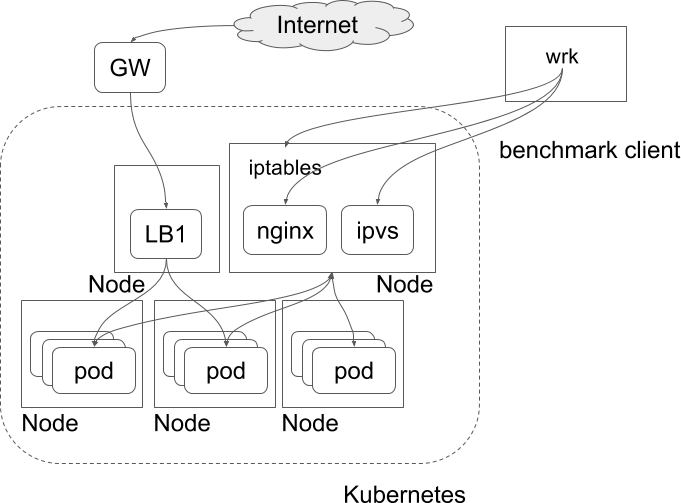
\includegraphics[width=0.8\columnwidth]{Figs/benchmark-schem}
  \vspace{1cm}
  \caption{Logical configuration.}
  \label{fig:benchmark-schem}
\end{subfigure}
  \vspace{1cm}

\begin{subfigure}[t]{\columnwidth}
  \centering
  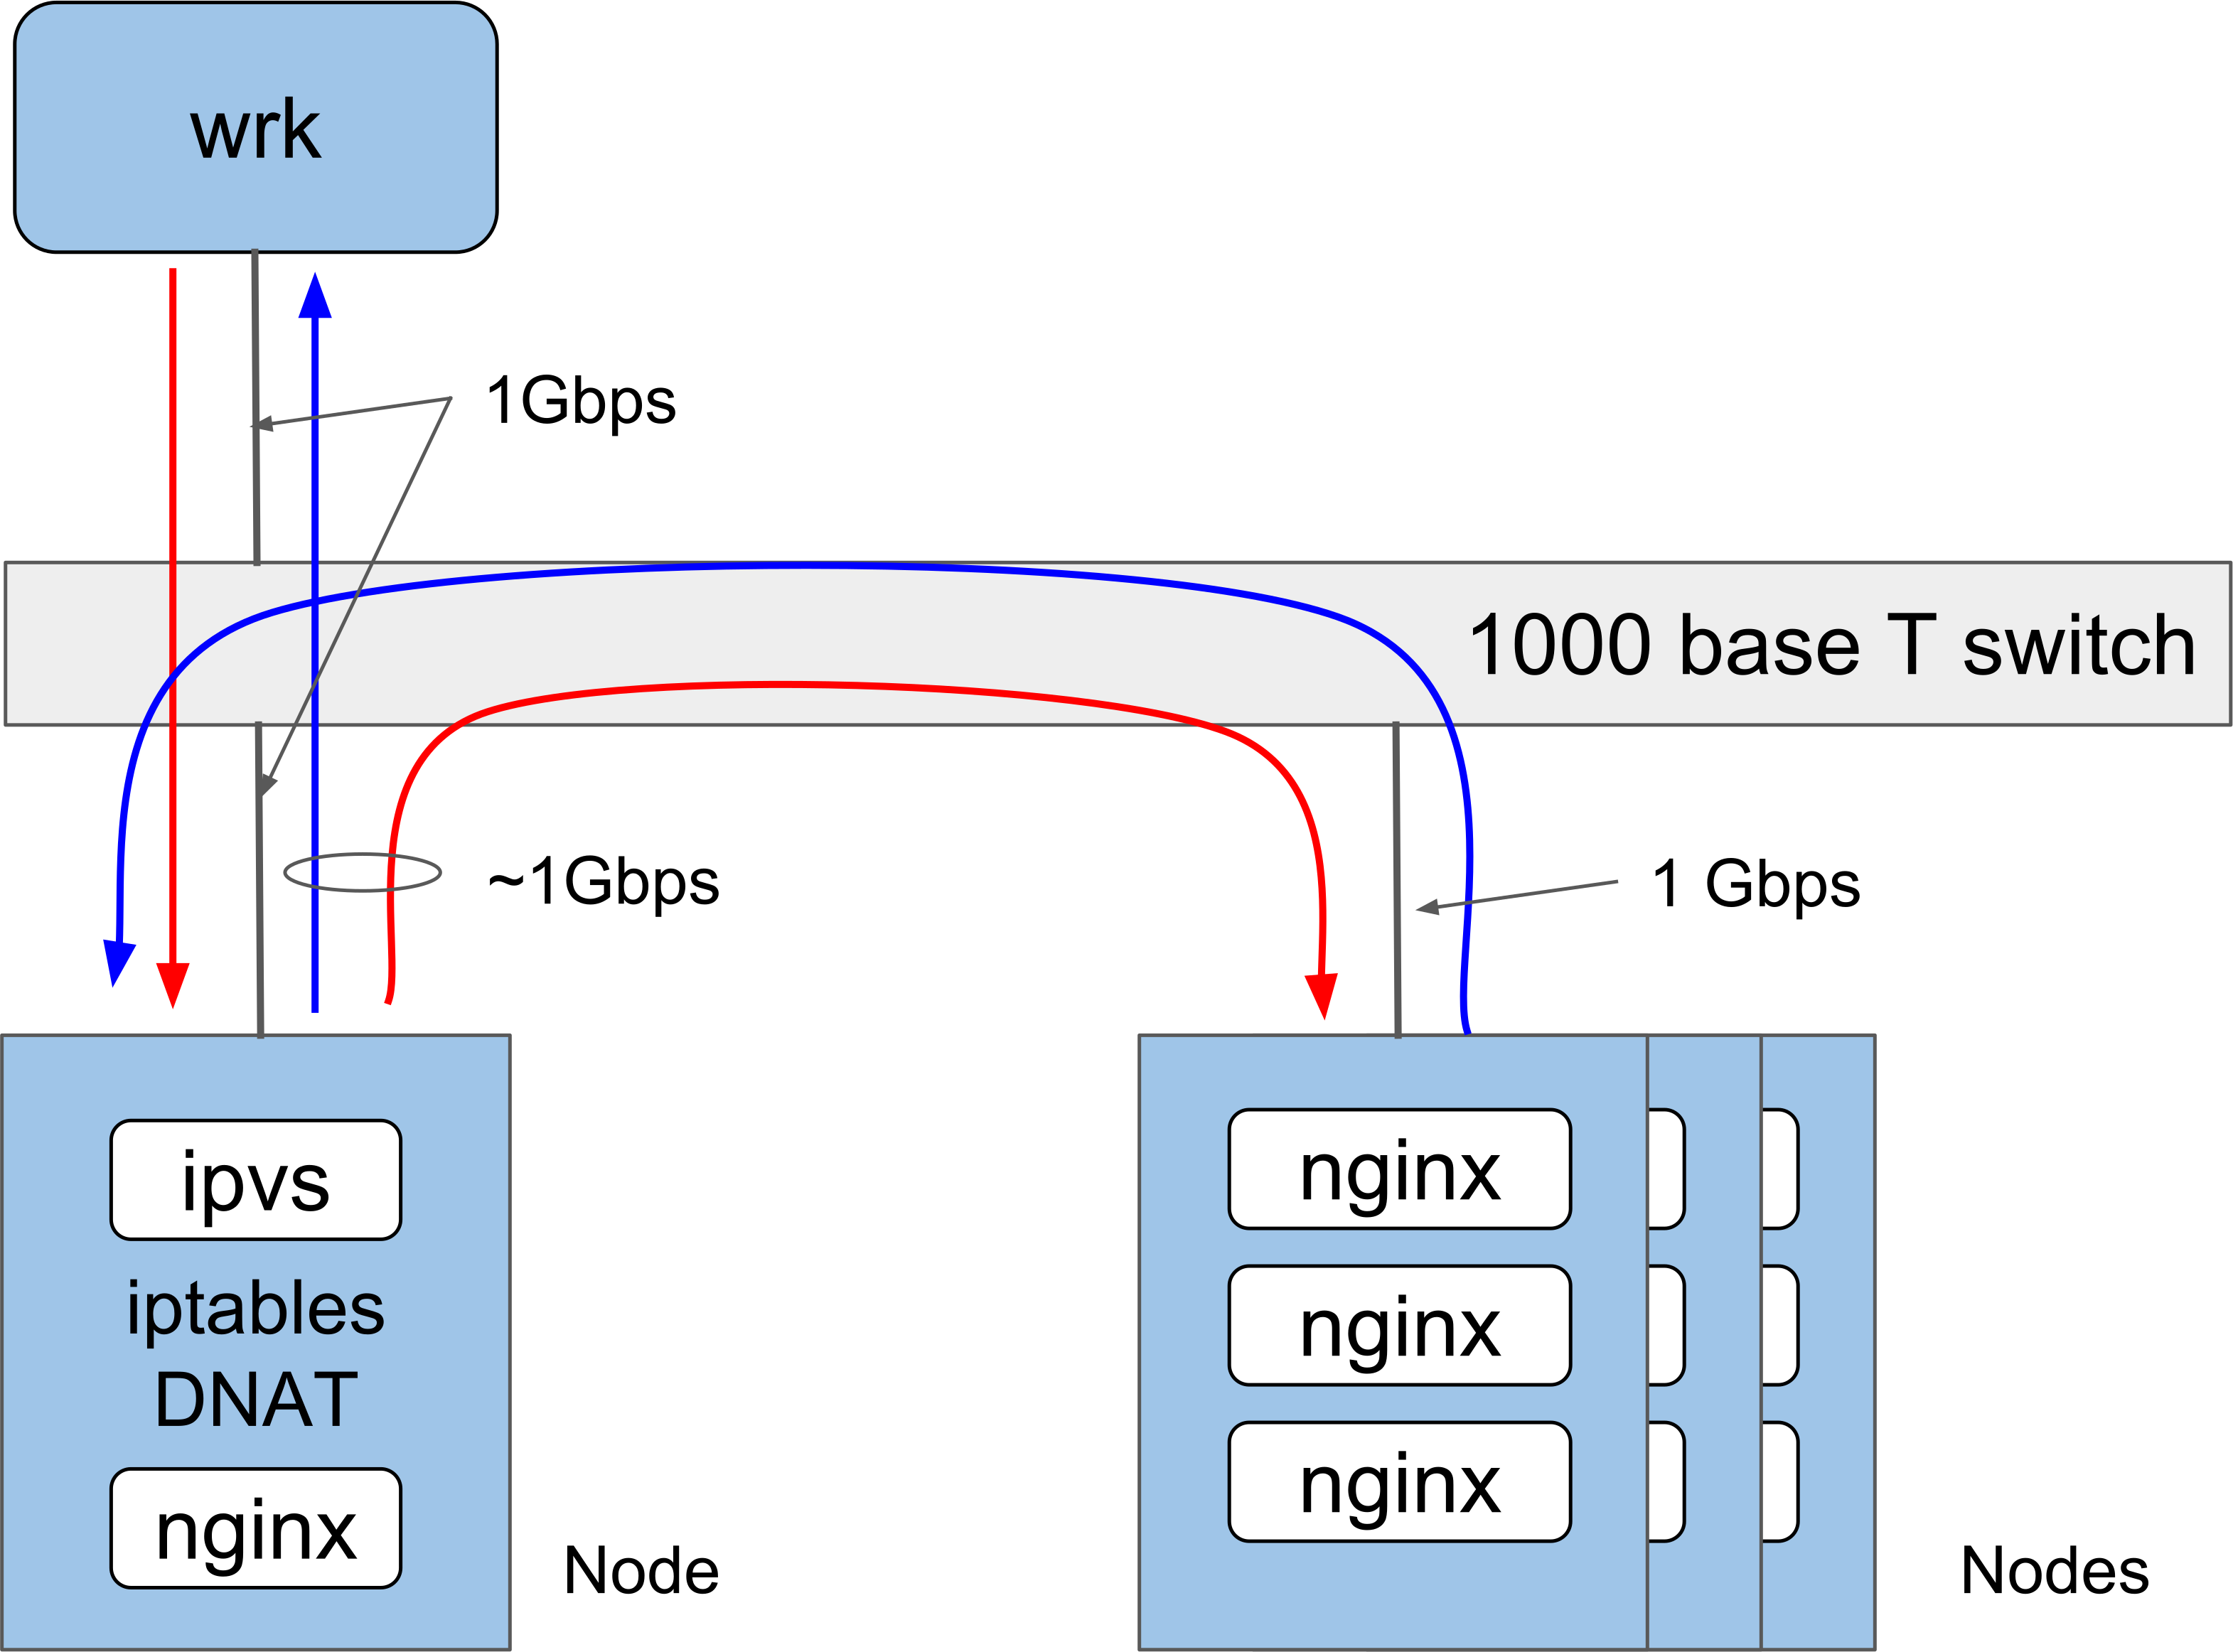
\includegraphics[width=0.8\columnwidth]{Figs/bench_1g}
  \vspace{1cm}
  \caption{Physical configuration.}
  \label{fig:bench_1g}
\end{subfigure}
  \caption{Benchmark setup. }
  \label{fig:benchmark-setup}
\end{figure}

Table~\ref{tab:bench_example} shows an example of the command-line for wrk and the corresponding output.
The command-line in Table~\ref{tab:bench_example} will generate 40 wrk program threads and allow those threads to send out a total of 800 concurrent HTTP requests over the period of 30 seconds.
The output example shows the information including per thread statistics, error counts, Request/sec and Transfer/sec.

\begin{table}[h]
  \centering
  \begin{tabular}{l}
    \hline
    \begin{minipage}{13cm}
      \begin{verbatim}

[Command line] 
 wrk -c800 -t40 -d30s http://172.16.72.2:8888/ 
-c: concurrency, -t: # of thread, -d: duration 

[Output example] 
 Running 30s test @ http://10.254.0.10:81/ 
  40 threads and 800 connections 
  Thread Stats   Avg      Stdev     Max   +/- Stdev 
    Latency    15.82ms   41.45ms   1.90s    91.90\% 
    Req/Sec     4.14k   342.26     6.45k    69.24\% 
  4958000 requests in 30.10s, 1.14GB read 
  Socket errors: connect 0, read 0, write 0, timeout 1 
Requests/sec: 164717.63 
Transfer/sec:     38.86MB 
      \end{verbatim}
    \end{minipage}
   \\ \hline
  \end{tabular}
  \caption{}
  \label{tab:bench_example}
\end{table}

Table~\ref{tab:hw_sw_spec} shows hardware and software configuration used in the experiments.
%Physical servers with the same specification are used for nodes(nginx, load balancer) and benchmark client.
All of the nginx web server pods are configured to return the IP address of the {\em pod}, in order to make them return a small HTTP content. This makes a relatively severe condition for load balancers. 
The size of the character string making up an IP address is limited to 15 bytes.
If the author had chosen the HTTP response size so that most of the IP packet resulted in maximum transmission unit(MTU), the performance would have been dominantly limited by the Ethernet bandwidth.
% However, since small HTTP responses are used, the auhtor could purely measure the load balancer performance.

\begin{table}[]
  \centering
  \begin{tabular}{ll}
    \hline 
    \multicolumn{2}{l}{[Hardware Specification]}   \\
    & CPU: Xeon E5-2450 2.10GHz (with 8 core, Hyper Threading) \\
    & Memory: 32GB \\
    & NIC: Broadcom BCM5720 Giga bit \\
    & (Node x 6, LB x 1, Client x 1) \\
    & \\
    \multicolumn{2}{l}{[Node Software]}  \\
    & OS: Debian 8.7, linux-3.16.0-4-amd64 \\
    & Kubernetes v1.10.6 \\
    & flannel v0.7.0 \\
    & etcd version: 3.0.15 \\
    & \\
    \multicolumn{2}{l}{[Container Software]}   \\
    & Keepalived: v1.3.2 (12/03,2016) \\
    & nginx : 1.11.1(load balancer), 1.13.0(web server) \\
    \hline
  \end{tabular}
  \caption{}
  \label{tab:hw_sw_spec}
\end{table}

For this experiment a total of eight servers are used; six servers for nodes, one for the load balancer and one for the benchmark client, with all having the same hardware specifications.
The software versions used for Kubernetes, web server and load balancer {\em pods} are also summarized in the Table~\ref{tab:hw_sw_spec}.
The hardware we used had eight physical CPU cores and a 1Gbps NIC with 4 rx-queues.

\subsection{Results}
\subsubsection{Effect of multicore proccessing}

\begin{figure}
  \centering
  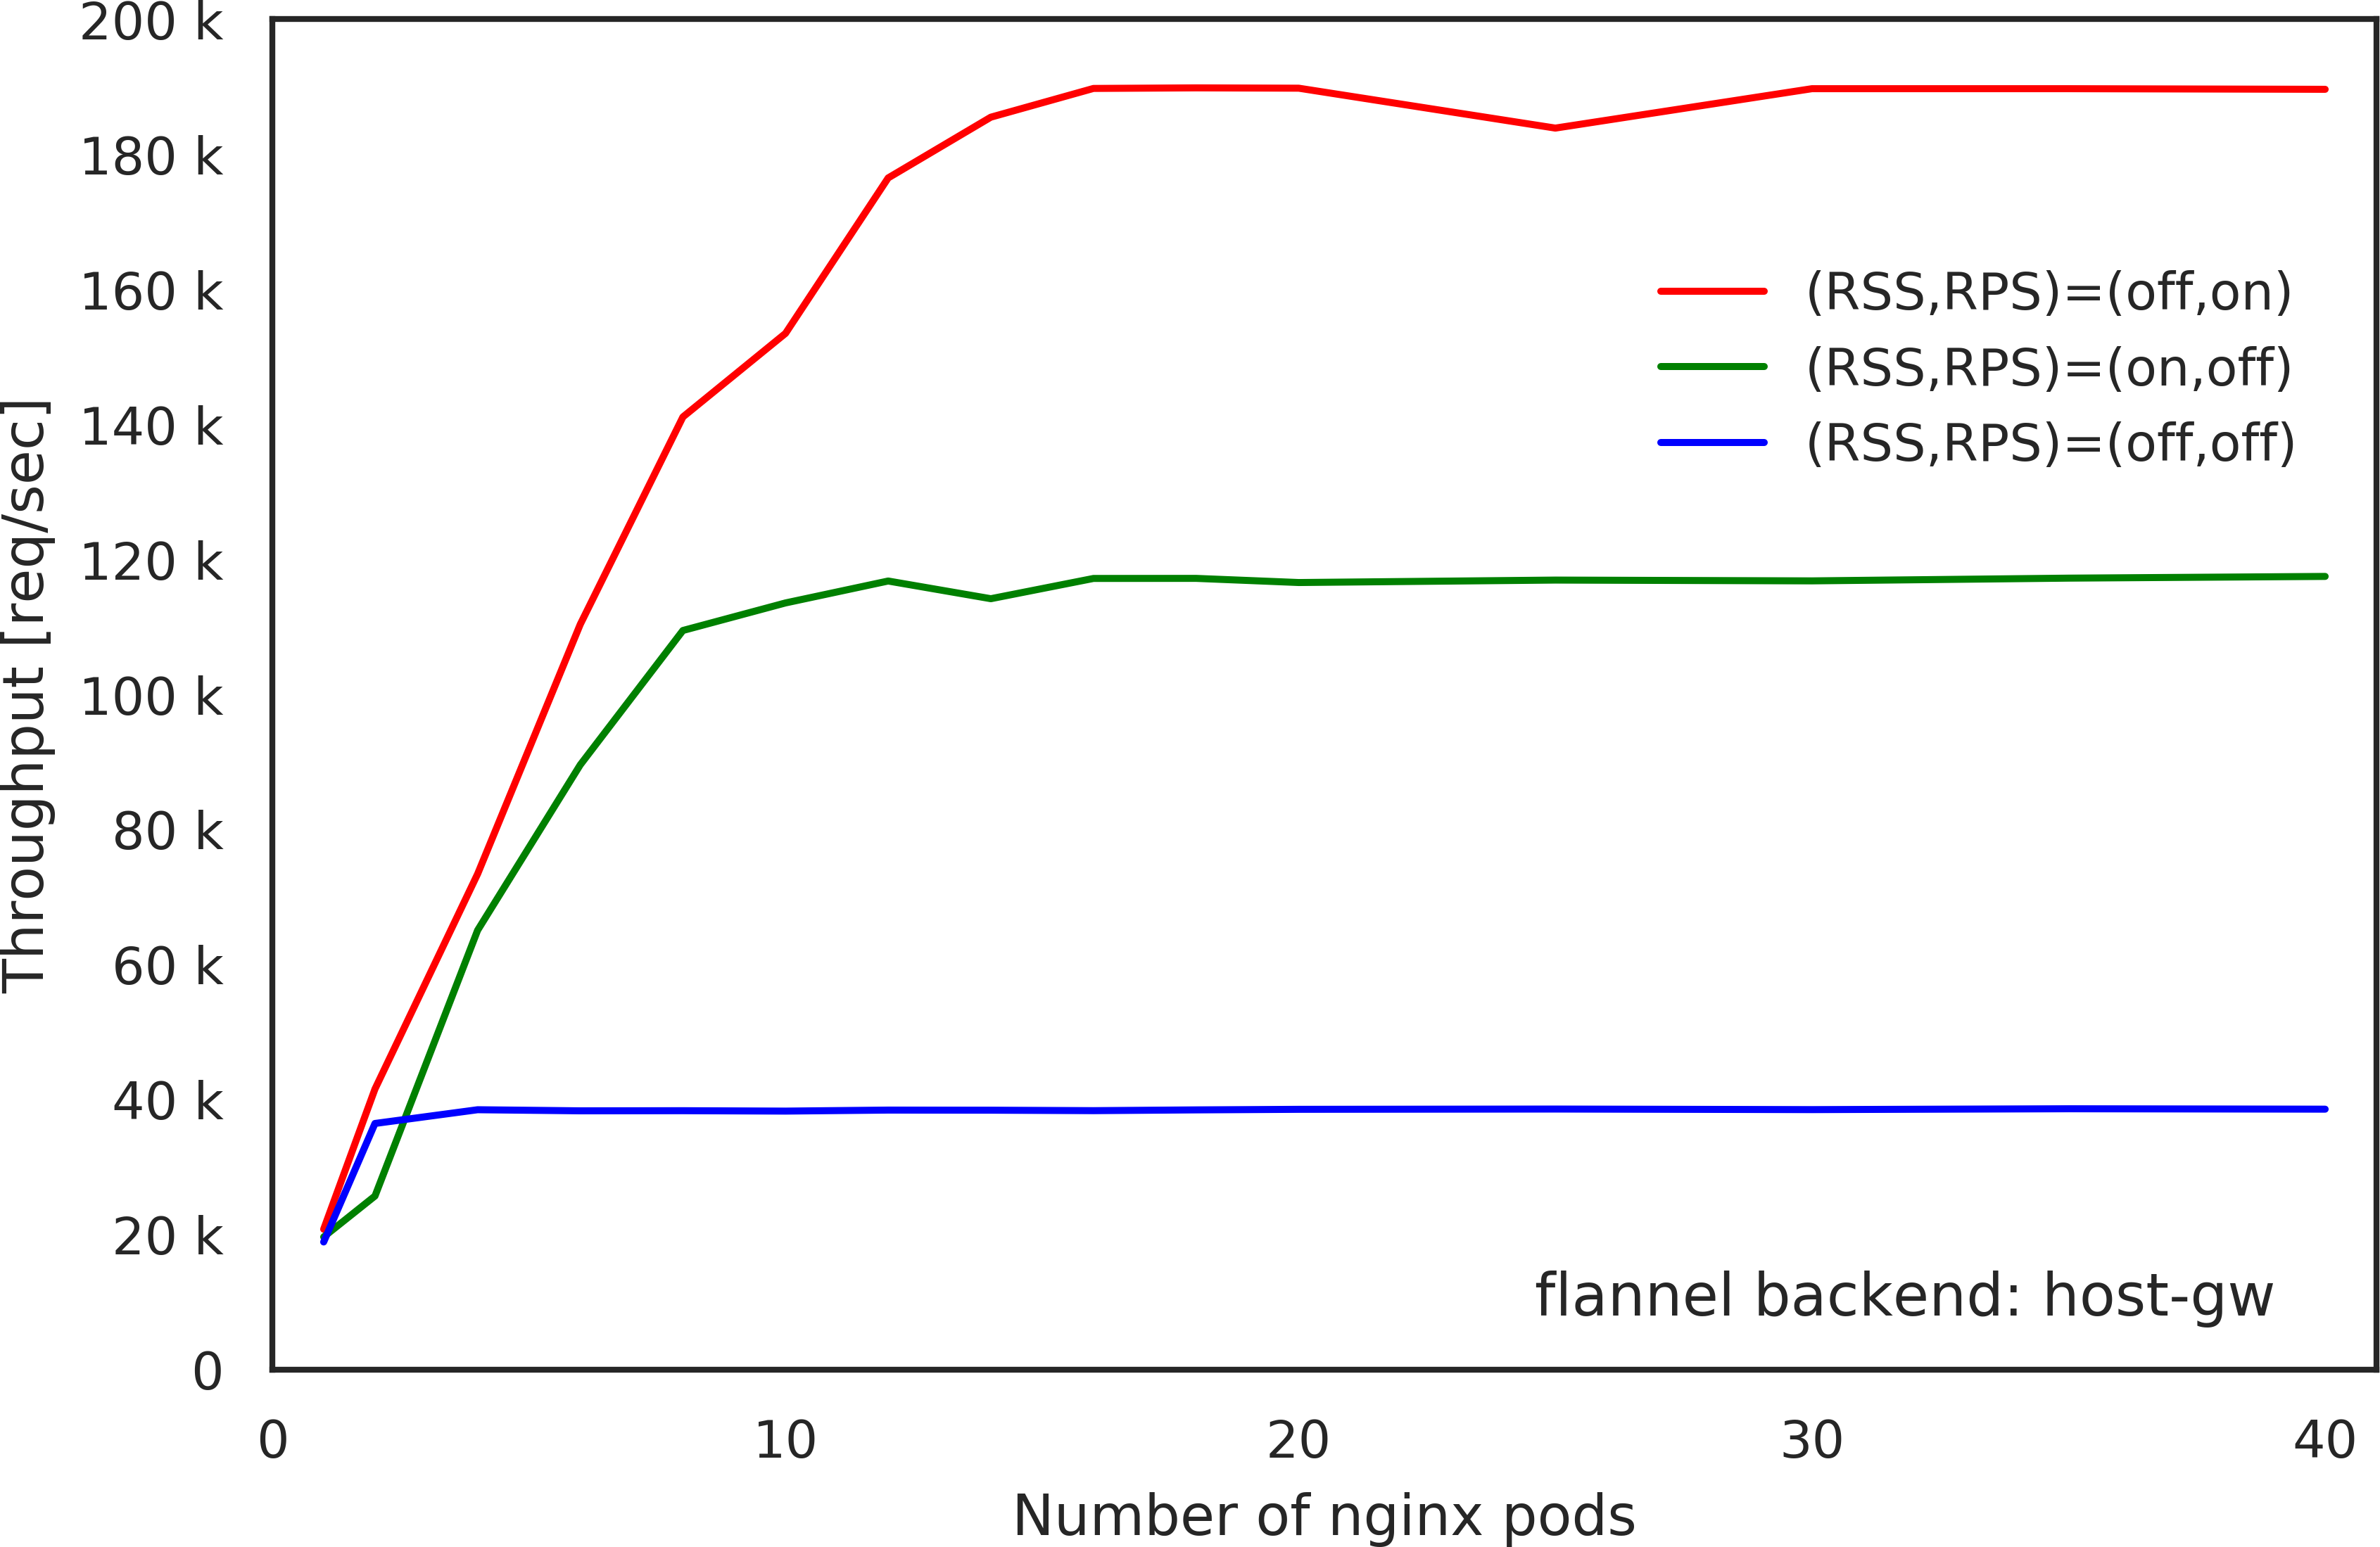
\includegraphics[width=0.8\columnwidth]{Figs/ipvs_mcore_proccessing}
  \caption{Effect of multicore proccessing on ipvs throughput.}
  \label{fig:ipvs_mcore_proccessing}
\end{figure}

Figure~\ref{fig:ipvs_mcore_proccessing} shows a result of throughput experiment with different multicore proccessing settings.
The following three RSS and RPS settings were compared: 
\begin{center}
  \centering
  \begin{minipage}{0.8\columnwidth}
\begin{verbatim}
(RSS, RPS) = (off, off)
           = (on , off)
           = (off, on )
\end{verbatim}
  \end{minipage}
\end{center}
%The host-gw mode of flannel backends is used as the overlay network.

The case with \enquote{(RSS, RPS) = (off, off)} means that multicore packet processing is completely disabled, i.e.,  all the incoming packets are processed by a single core.
The \enquote{(RSS, RPS) = (on, off)} means that the interrupt handling and the following IP protocol processing are performed on four of the CPU cores by assigning four rx-queues to those cores. In this case four of the eight CPU cores are utilized.
The \enquote{(RSS, RPS) = (off, on)} means that a single core handles all of the interrupts from the NIC then the following IP processings are performed on the other cores. In this case, all of the eight CPU cores are utilized.

We can see a general trend in which the throughput linearly increases as the number of nginx {\em pod}s increases and then it eventually saturates.
The saturated throughput levels indicate the maximum performance level of the ipvs load balancer.
The maximum performance levels depend on the (RSS, RPS) settings.
From the results in this figure, it can be seen that if we turn off multicore packet processing,
{\it i.e.}, when \enquote{(RSS, RPS) = (off, off)}, performance degrades significantly.
%In this case, the performance bottleneck is primarily due to packet processing in a single core.

If we compare the results for the cases when \enquote{(RSS, RPS) = (on, off)} and \enquote{(RSS, RPS) = (off, on)},
the latter is better than the former.
It is clear that the case that utilizes all of the CPU cores better performs than the case with only four CPU cores utilized. 

\begin{figure}[h]
  \centering
  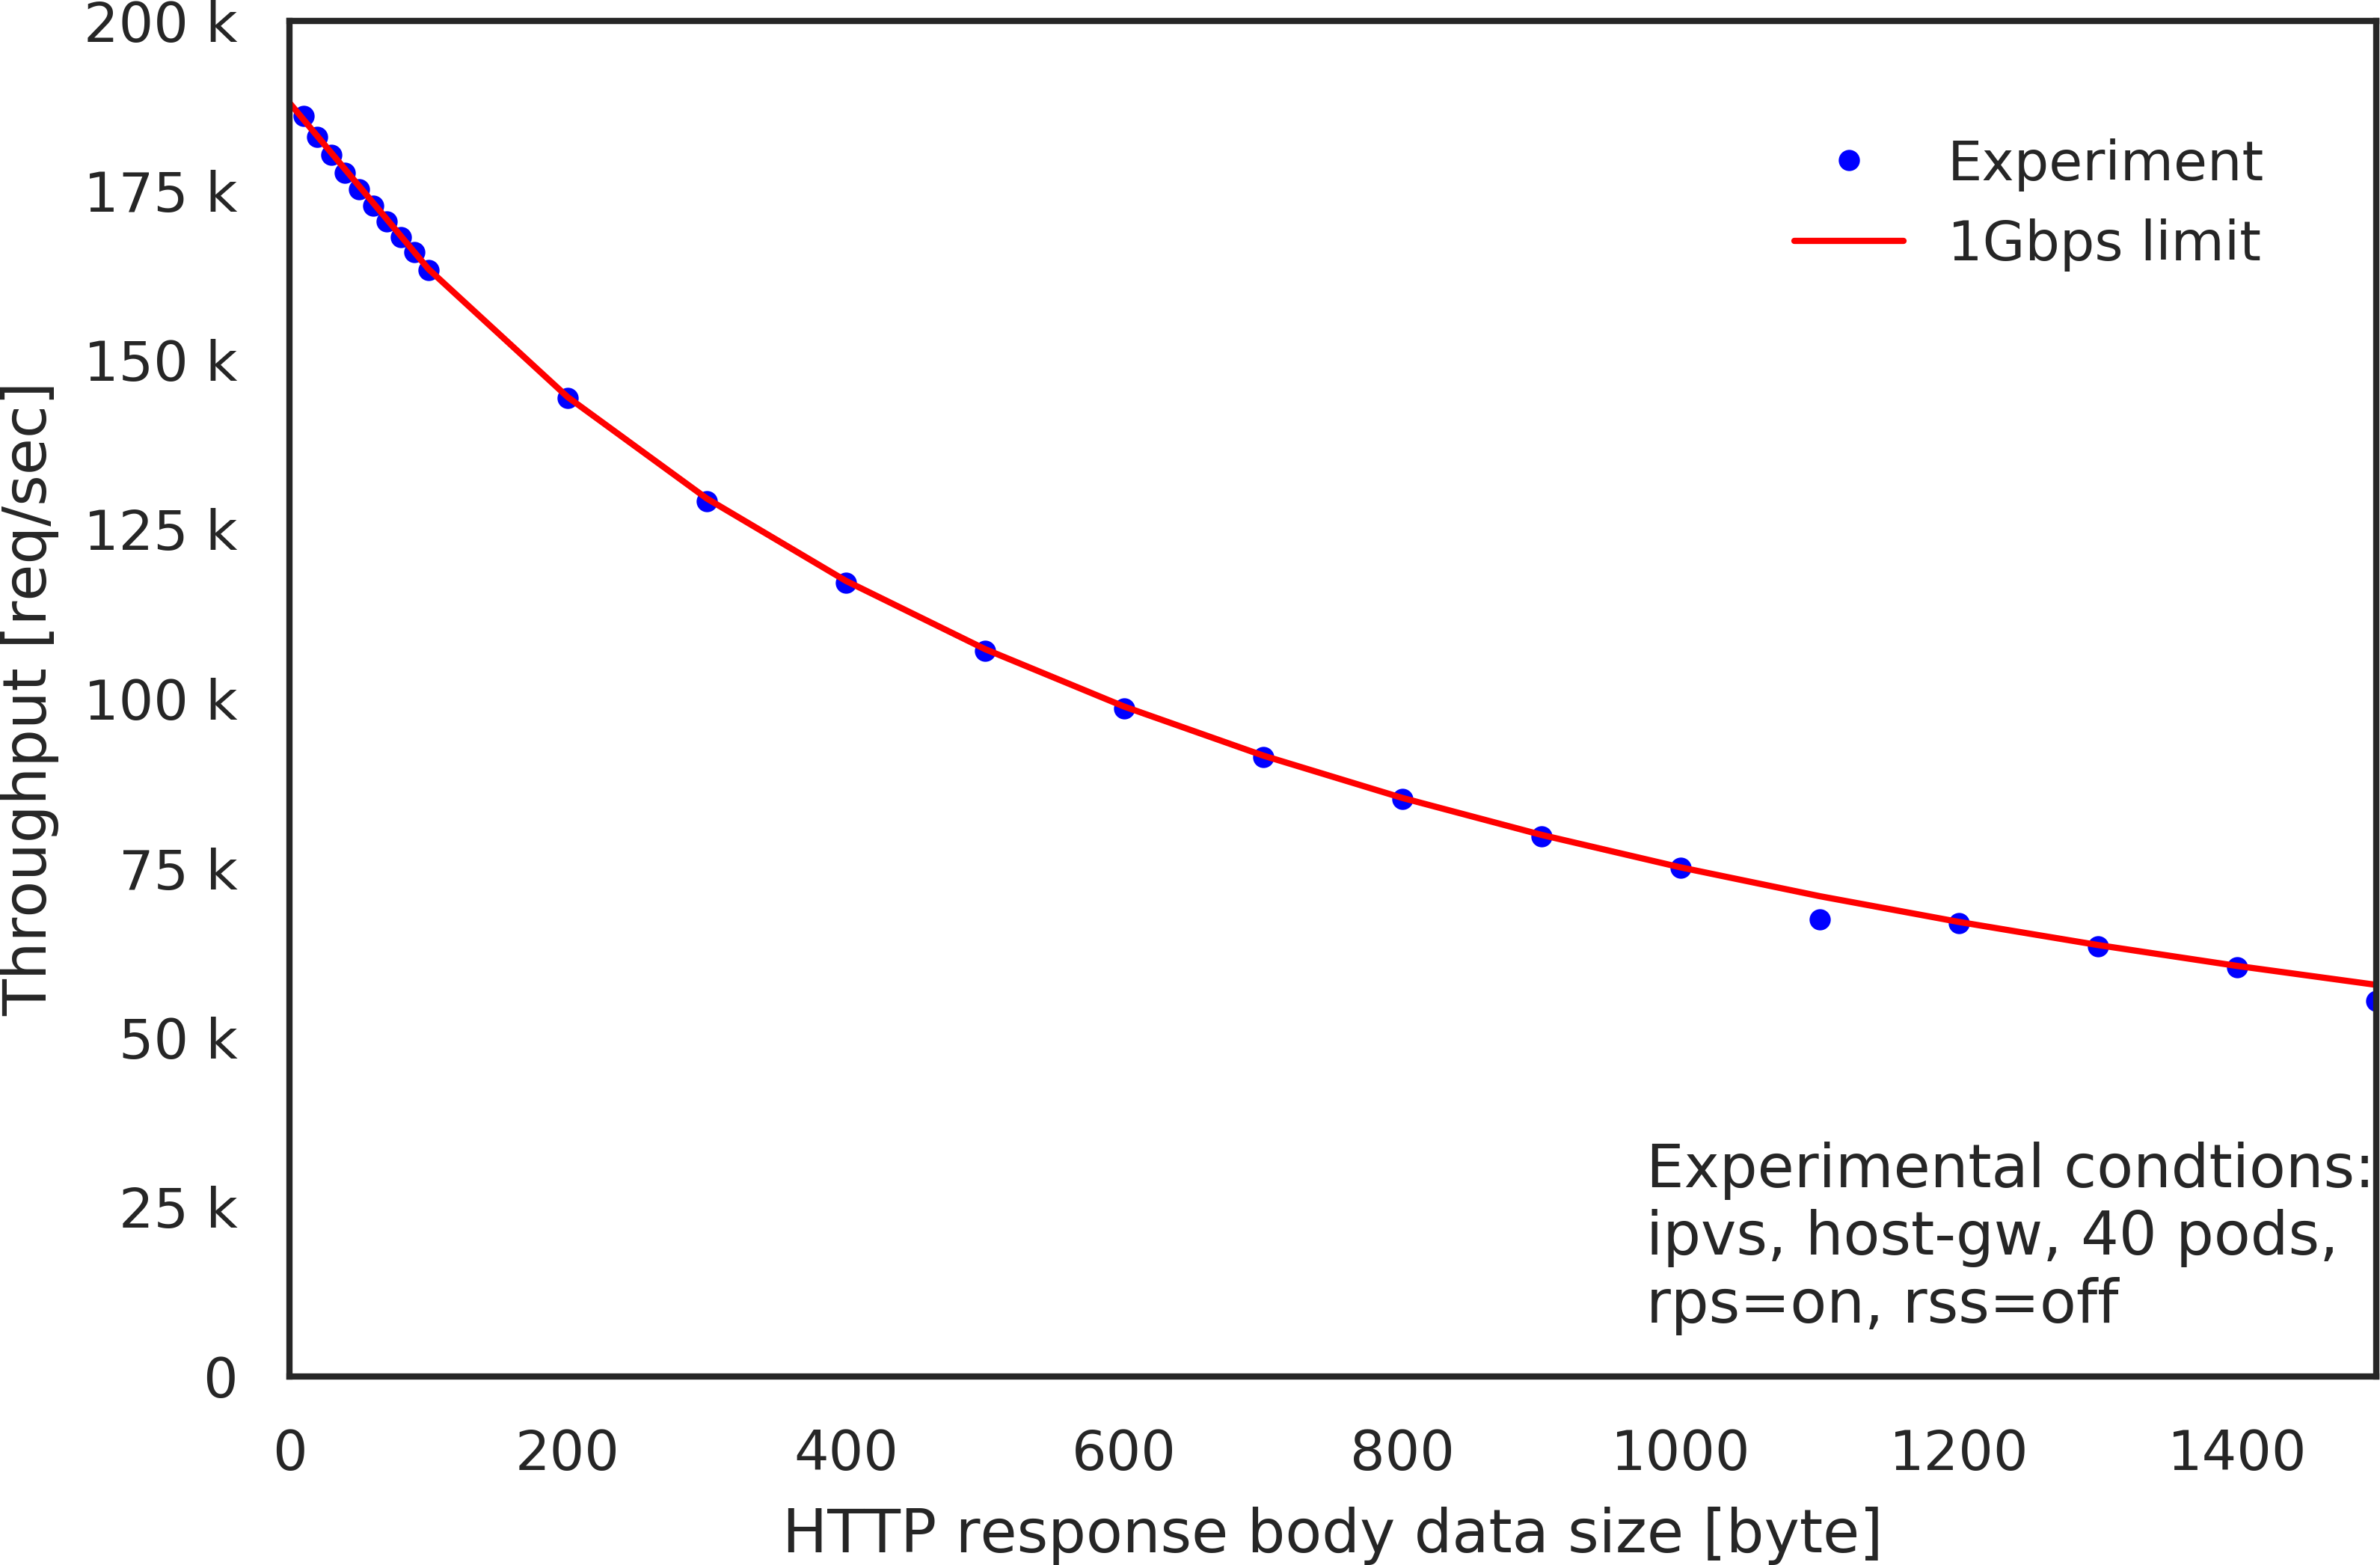
\includegraphics[width=0.8\columnwidth]{Figs/tp_limit_1gbps}
  \caption{Performance limit due to 1Gbps bandwidth}
  \label{fig:performance_limit}
\end{figure}

At first, it was not clear what caused the performance limit for the case when \enquote{(RSS, RPS) = (off, on)},
the author thought it was due to the insufficient CPU performance.
However, that was not the case in the conditions of the experiment; it turned out to be due to the 1Gbps bandwidth.
A packet level analysis using tcpdump\cite{jacobson1989tcpdump} revealed that 665.36 bytes of extra HTTP headers,
TCP/IP headers and ethernet frame headers are needed for each request in the case of the wrk benchmark program(Appendix~\ref{appendix:performance_limit}).
This results in the upper limit of 184,267 [req/sec] when the date size of HTTP response body is 13 byte, which agrees well with the performance limit for the case when \enquote{(RSS, RPS) = (off, on)} in Figure~\ref{fig:ipvs_mcore_proccessing}.
Figure~\ref{fig:performance_limit} shows the theoretical upper limit of the performance level for 1Gbps ethernet together with actual benchmark results for the range of larger data sizes, and they agree very well.
Therefore it can be said that when \enquote{RPS = on}, ipvs performance is limited by 1Gbps bandwidth.
The author regarded that \enquote{(RSS, RPS) = (off, on)} is the best setting in our experimental conditions, and used this setting throughout this thesis unless explicitly stated otherwise.


\FloatBarrier

\subsubsection{Effect of overlay network}

\begin{figure}[h]
  \centering
  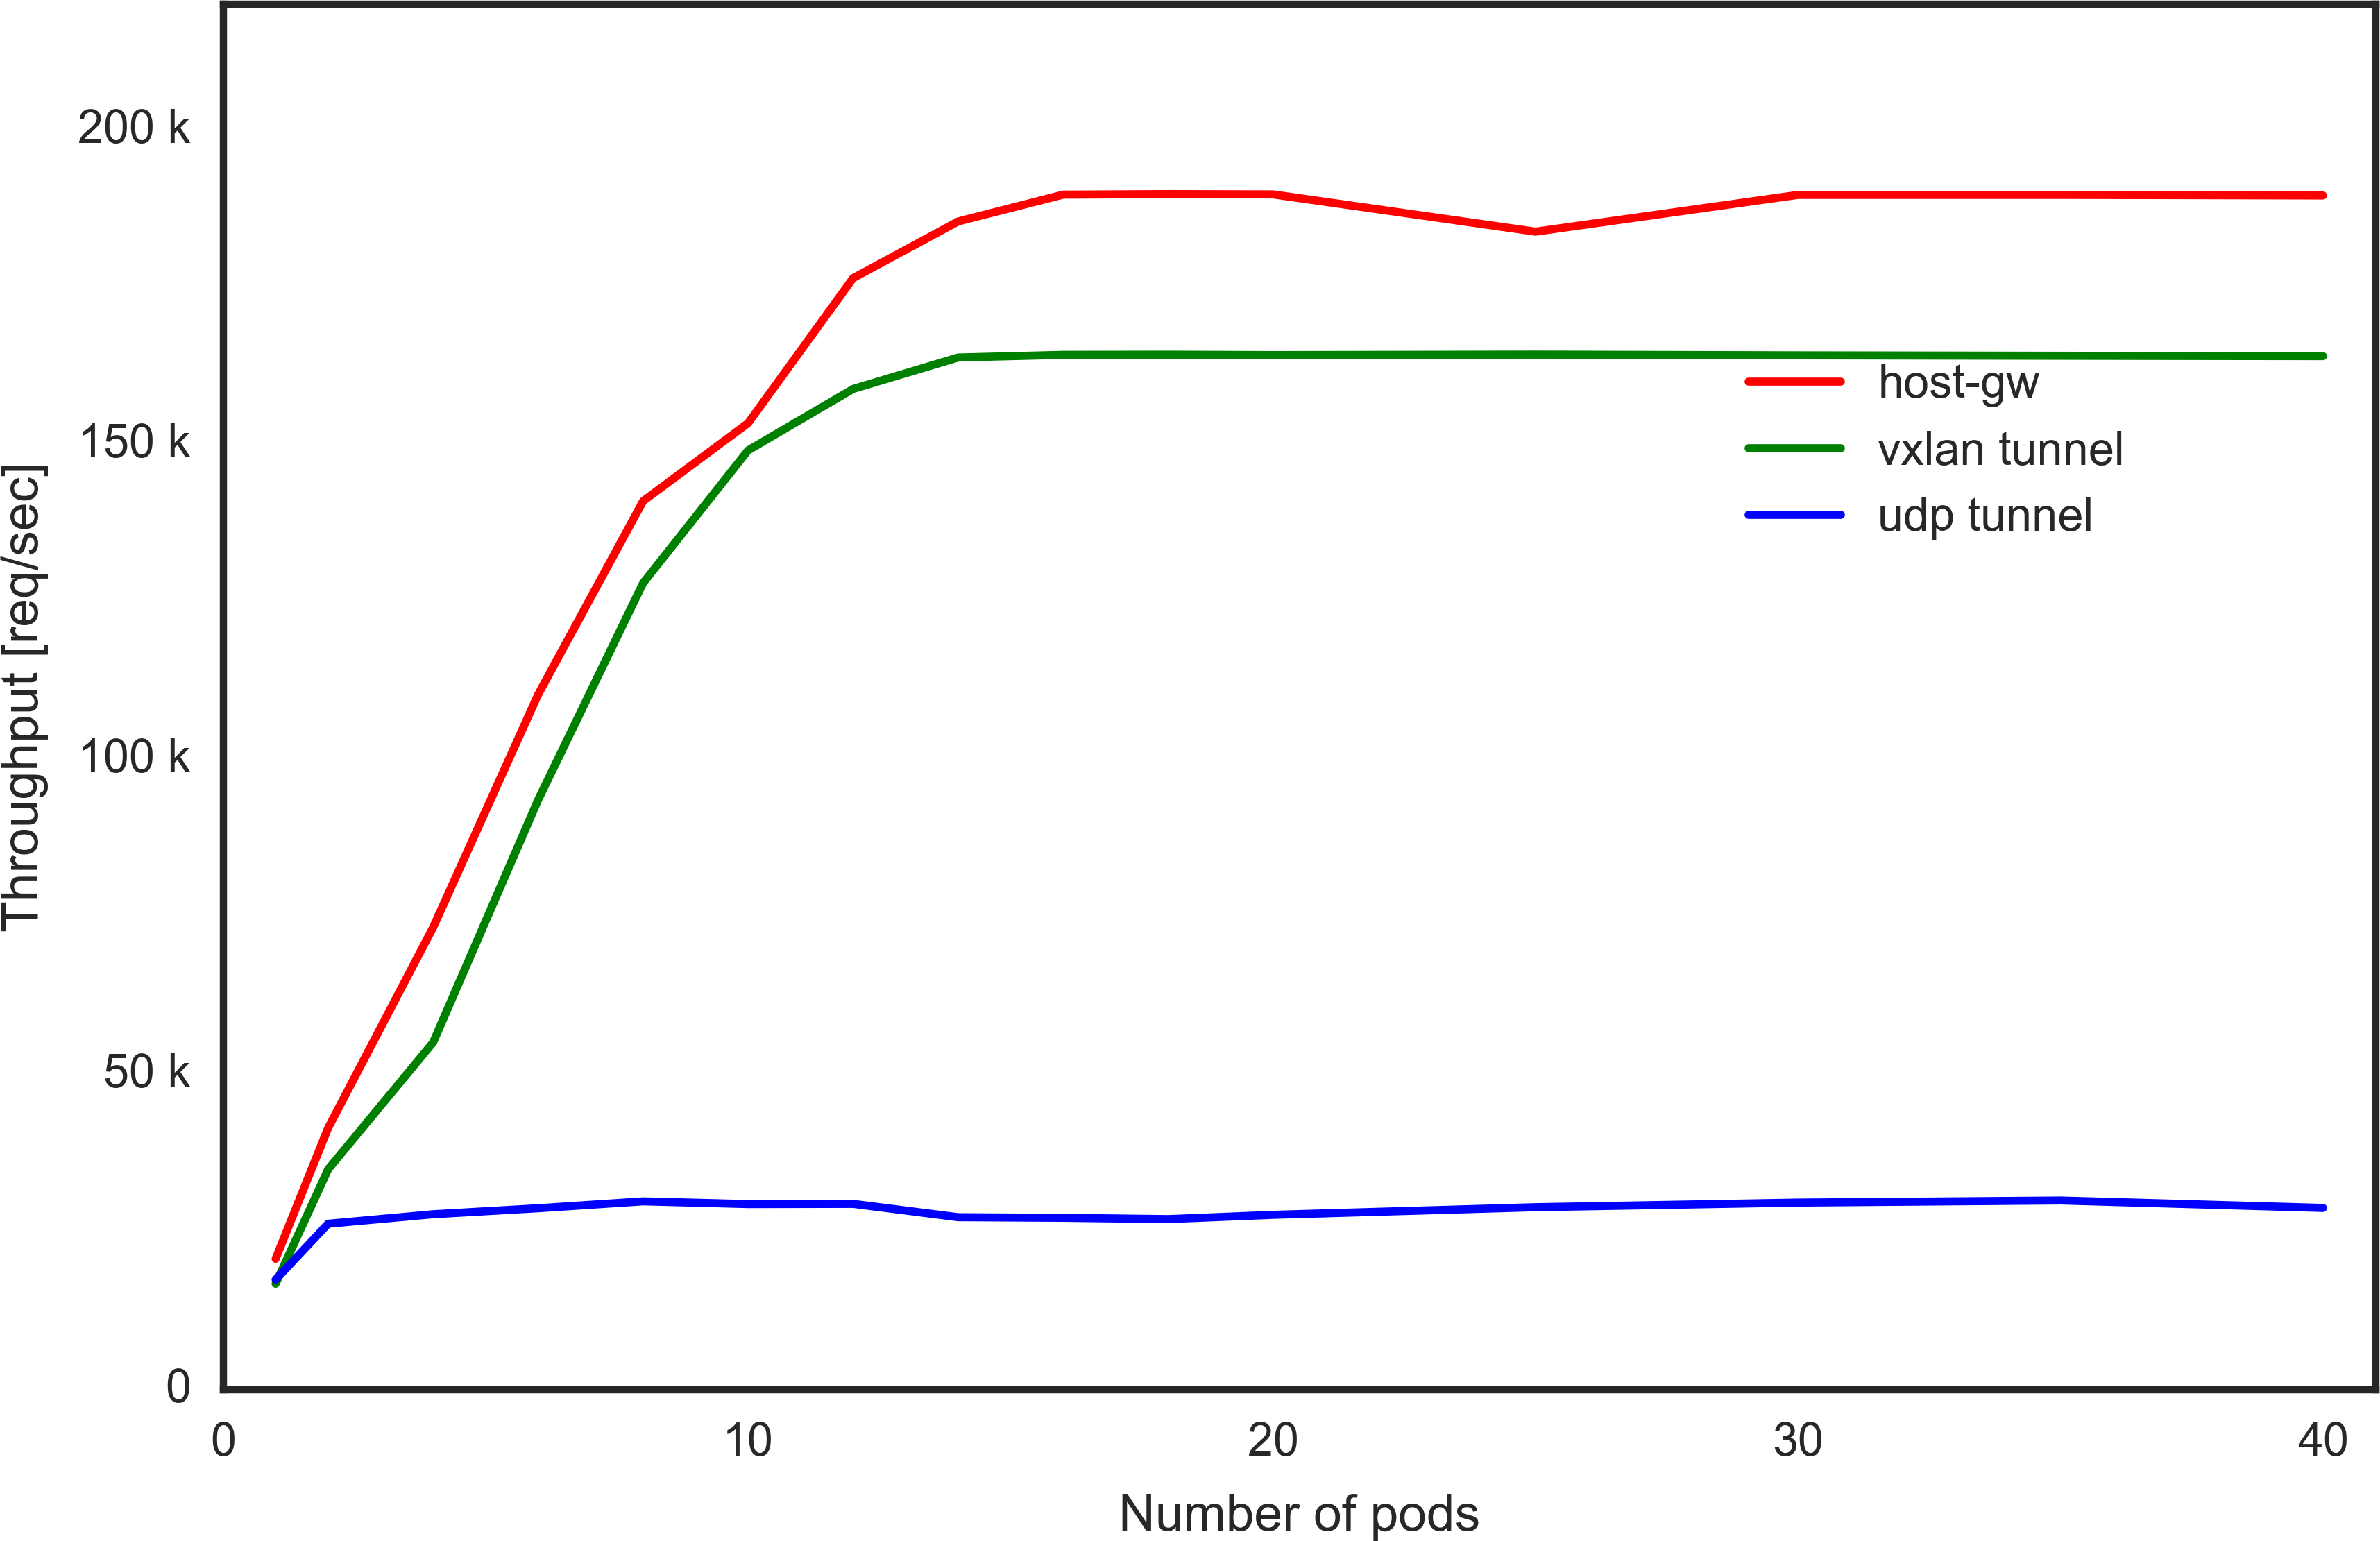
\includegraphics[width=0.8\columnwidth]{Figs/ipvs_flannel_mode}
  \caption{Effect of flannel backend modes on ipvs throughput.}
  \label{fig:ipvs_flannel_mode}
\end{figure}

Figure~\ref{fig:ipvs_flannel_mode} shows the ipvs throughput results for different overlay network settings.
As for the overlay network, the author used the flannel and measured the performance levels for flannel's three backend modes, host-gw, vxlan and udp.
Except for the udp backend mode case, we can see the trend in which the throughput linearly increases as the number of nginx {\em pod} increases and then it eventually saturates.
The saturated throughput levels indicate the maximum performance levels of the ipvs load balancer.
If we compare the performance levels among the flannel backend modes types, 
the host-gw mode where no encapsulation is conducted shows the highest performance level,
followed by the vxlan mode where the Linux kernel encapsulate the Ethernet frame.
The udp mode where flanneld itself encapsulate the IP packet shows significantly lower performances levels.
The author considers the host-gw mode is the best, the vxlan tunnel the second best and the udp tunnel mode unusable.
As is shown here, overlay network settings greately affect the performance level.
The author used host-gw mode for most of the experiments conducted in on-premise data centers and vxlan mode for the experiments conducted in cloud environments.  


\FloatBarrier

\subsubsection{Comparison of different load balancer}

\begin{figure}[htb]
  \centering
  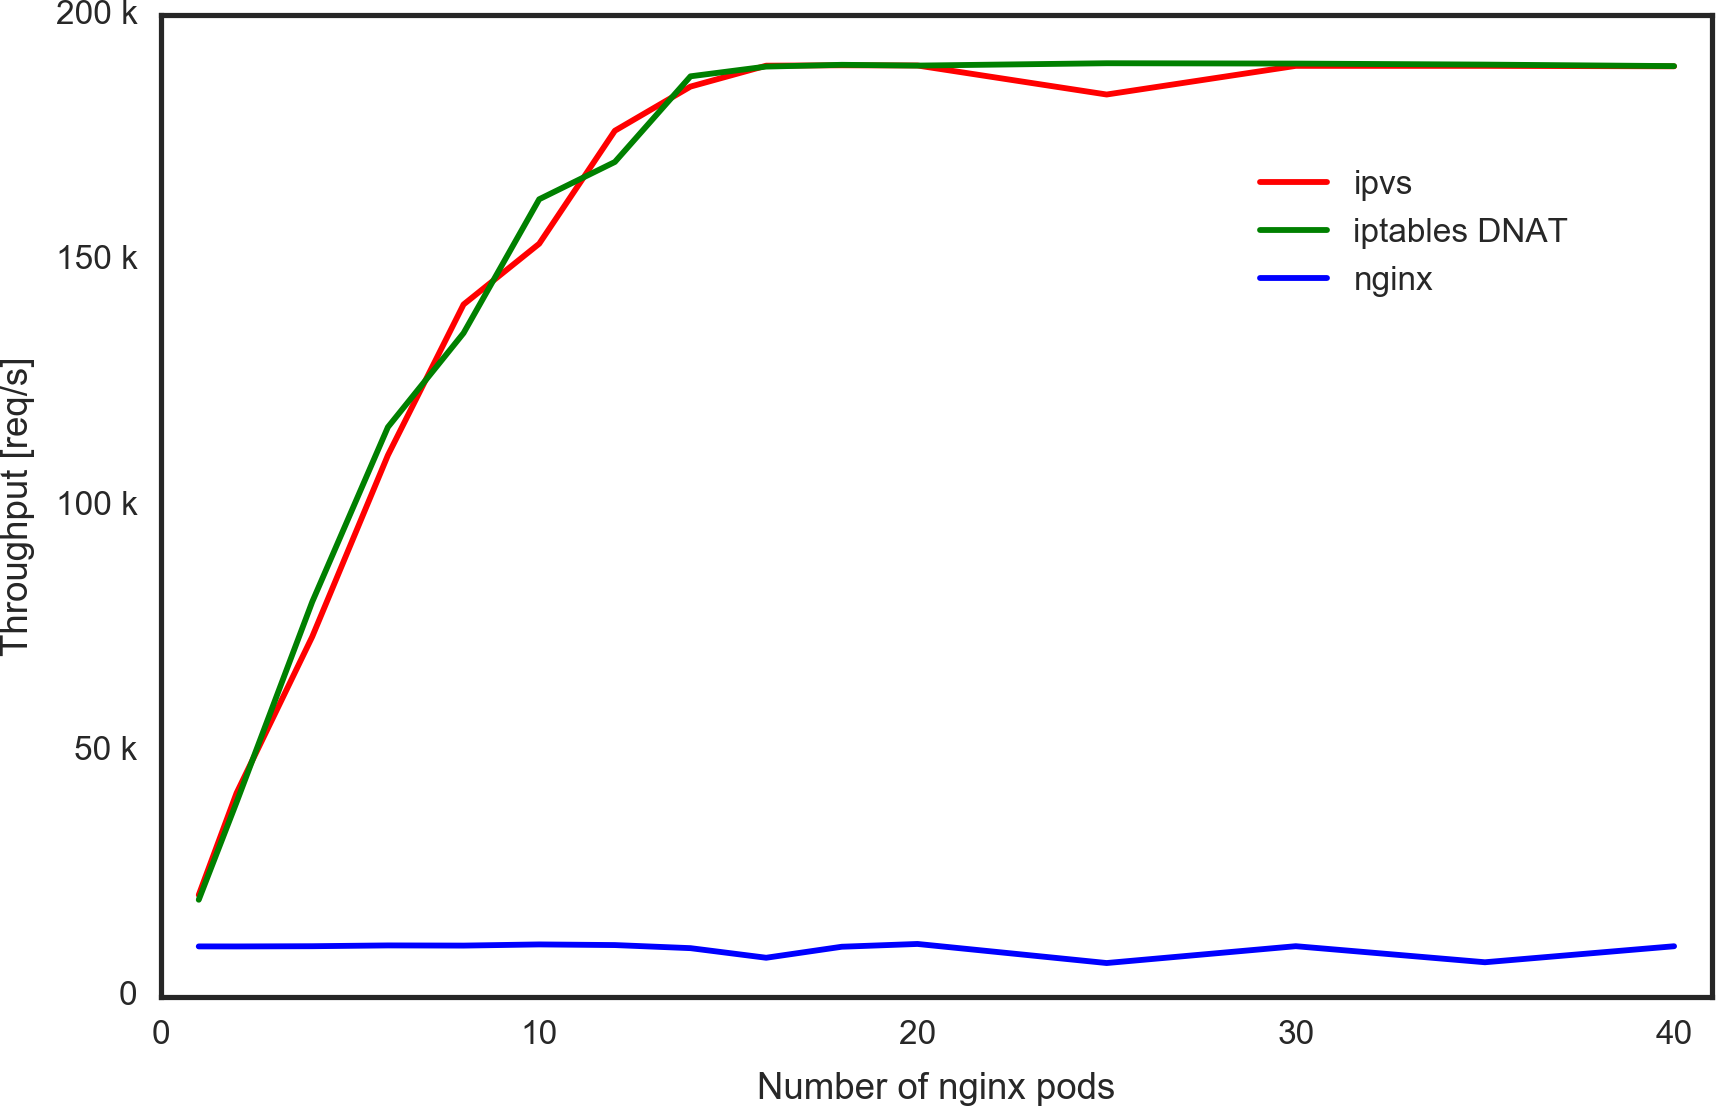
\includegraphics[width=0.8\columnwidth]{Figs/ipvs-iptables-nginx}
  \caption{Throughput comparison between ipvs, iptables DNAT and nginx.}
  \label{fig:ipvs-iptables-nginx}
\end{figure}

\begin{figure}[htb]
  \centering
  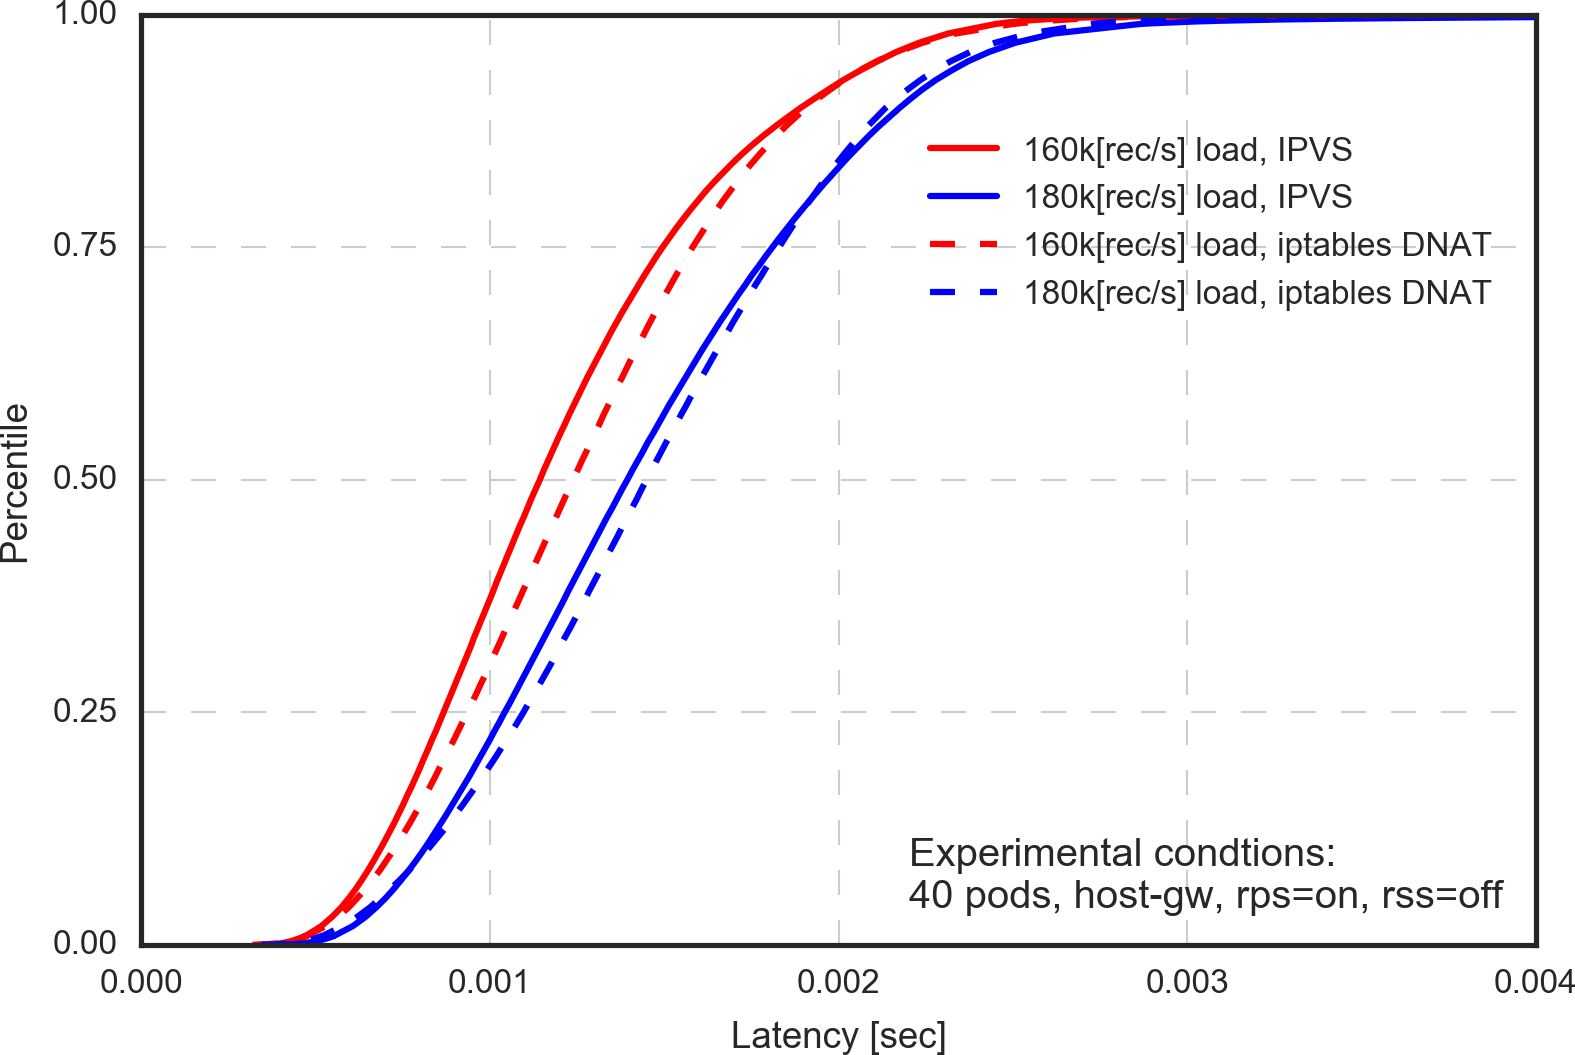
\includegraphics[width=0.8\columnwidth]{Figs/latency_cdf_rps_40pods}
  \caption{Latency cumulative distribution function.}
  \label{fig:latency_cdf_rps_40pods}
\end{figure}

Figure~\ref{fig:ipvs-iptables-nginx} compares the performance measurement results for different load balancer ipvs, iptables DNAT, and nginx.
The proposed ipvs load balancer exhibits almost equivalent performance levels as the iptables DNAT based load balancer. 
The nginx based load balancer shows no performance improvement even though the number of the nginx web server {\em pods} is increased.
It is understandable because the performance of the single nginx as a load balancer is expected to be similar to the performance as a web server.

Figure~\ref{fig:latency_cdf_rps_40pods} compares Cumulative Distribution Function(CDF) of the load balancer latency at the two constant loads, 160K[req/sec] and 180K[req/sec] for ipvs and iptables DNAT.
We can see that the latencies are a little bit smaller for ipvs.
For example, the median values at 160K[req/sec] load for ipvs and iptables DNAT are, 1.14 msec and 1.24 msec, respectively.
Also, at 160K[req/sec], they are 1.39 msec and 1.45 msec, respectively.
These may not be considered a significant difference; however, we can at least say that our proposed load balancer is as good as iptables DNAT.
So, to conclude this section, the containerized ipvs load balancer showed equivalent performance levels with the iptables DNAT load-balancing function that is used in Kubernetes cluster.

\FloatBarrier

\subsubsection{L3DSR using ipvs tun}

The performance levels of ipvs and iptables DNAT have been limited by 1 Gbps bandwidth.
This can be alleviated in the case of ipvs by using so-called Layer 3 Direct Server Return(l3dsr) setup.
Figure~\ref{fig:bench_1g_l3dsr} shows the schematic diagram illustrating packet flow for the HTTP request packet(the red arrows) and response packet(the blue arrow).

The ipvs has the mode called ipvs-tun.
When the ipvs-tun send out the packets to real servers, it encapsulates the original packet in ipip tunneling packet that is destined to real servers.
The real server receives the packet on a tunl0 device and decapsulates the ipip packet, revealing the original packet.
Since the source IP address of the original packet is maintained, the returning packets are sent directly toward the benchmark client.
In this scheme, the returning packets do not consume the bandwidth nor the CPU power of the load balancer node.

The iptables DNAT does not have the functions that enable L3DSR settings.
Therefore this one of the benefits of the ipvs load balancer.

\begin{figure}[h]
  \centering
  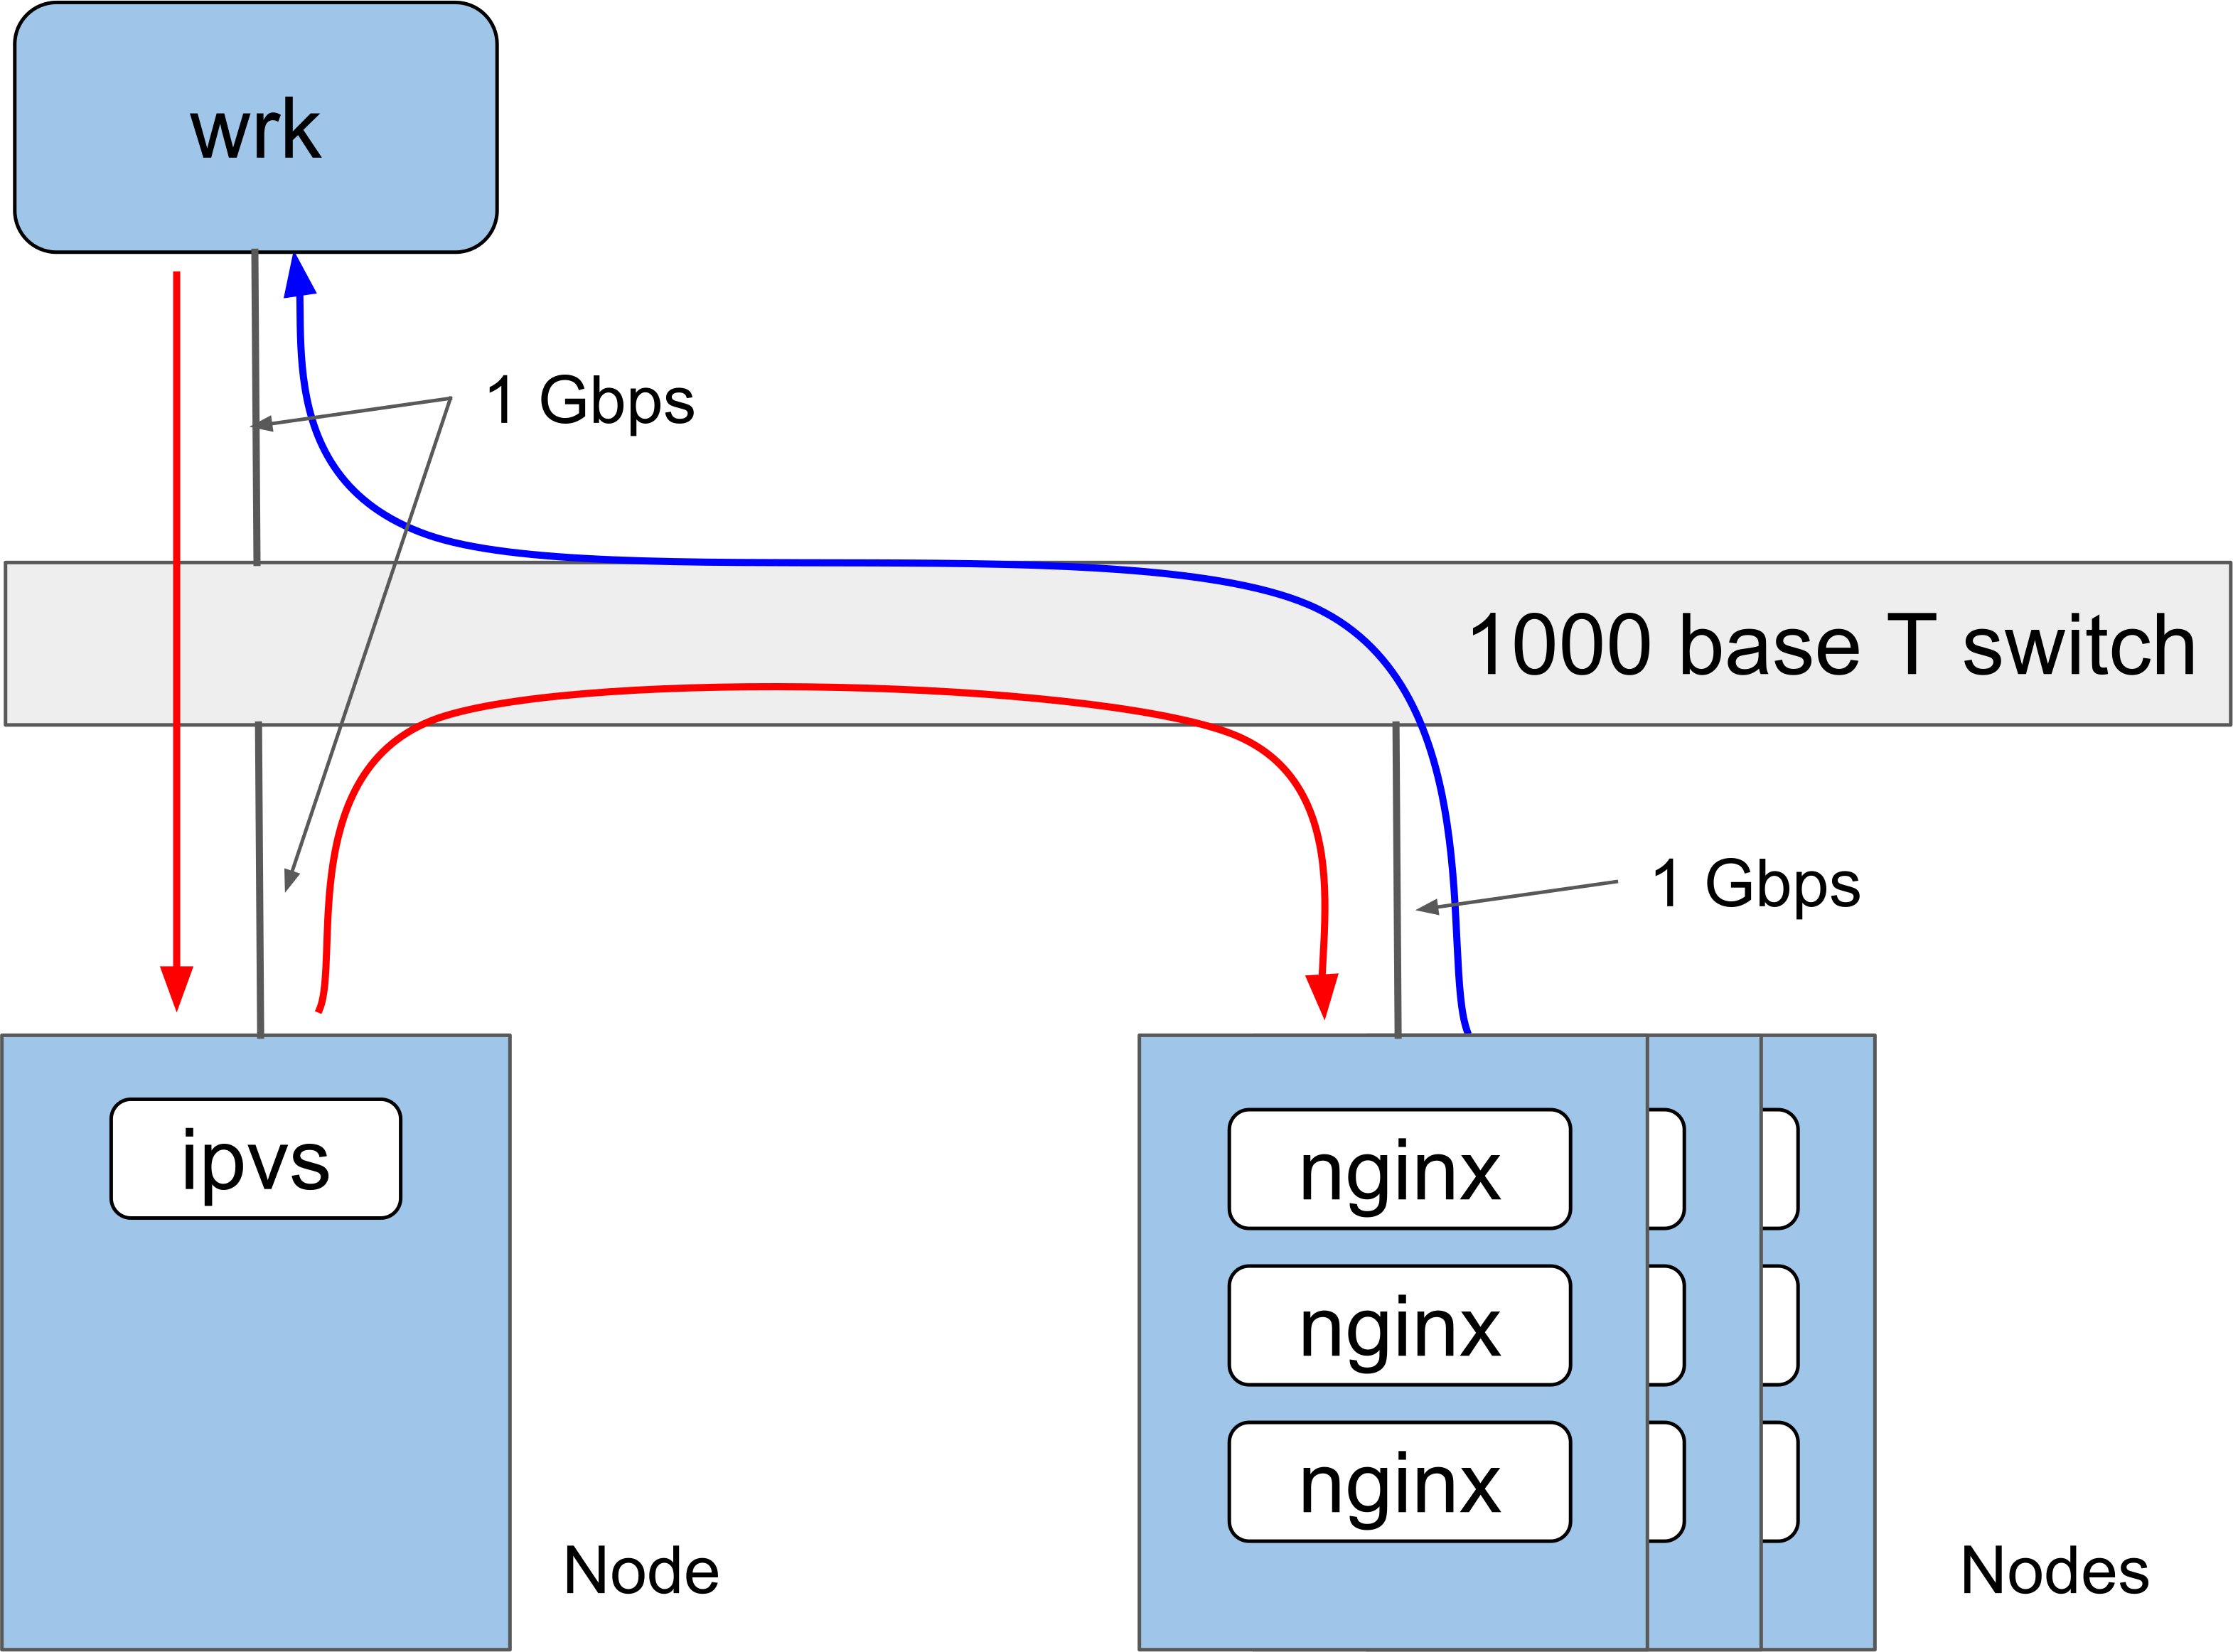
\includegraphics[width=0.8\columnwidth]{Figs/bench_1g_l3dsr}
  \caption{Physical configuration for L3DSR experiment.}
  \label{fig:bench_1g_l3dsr}
\end{figure}

\begin{figure}[h]
  \centering
  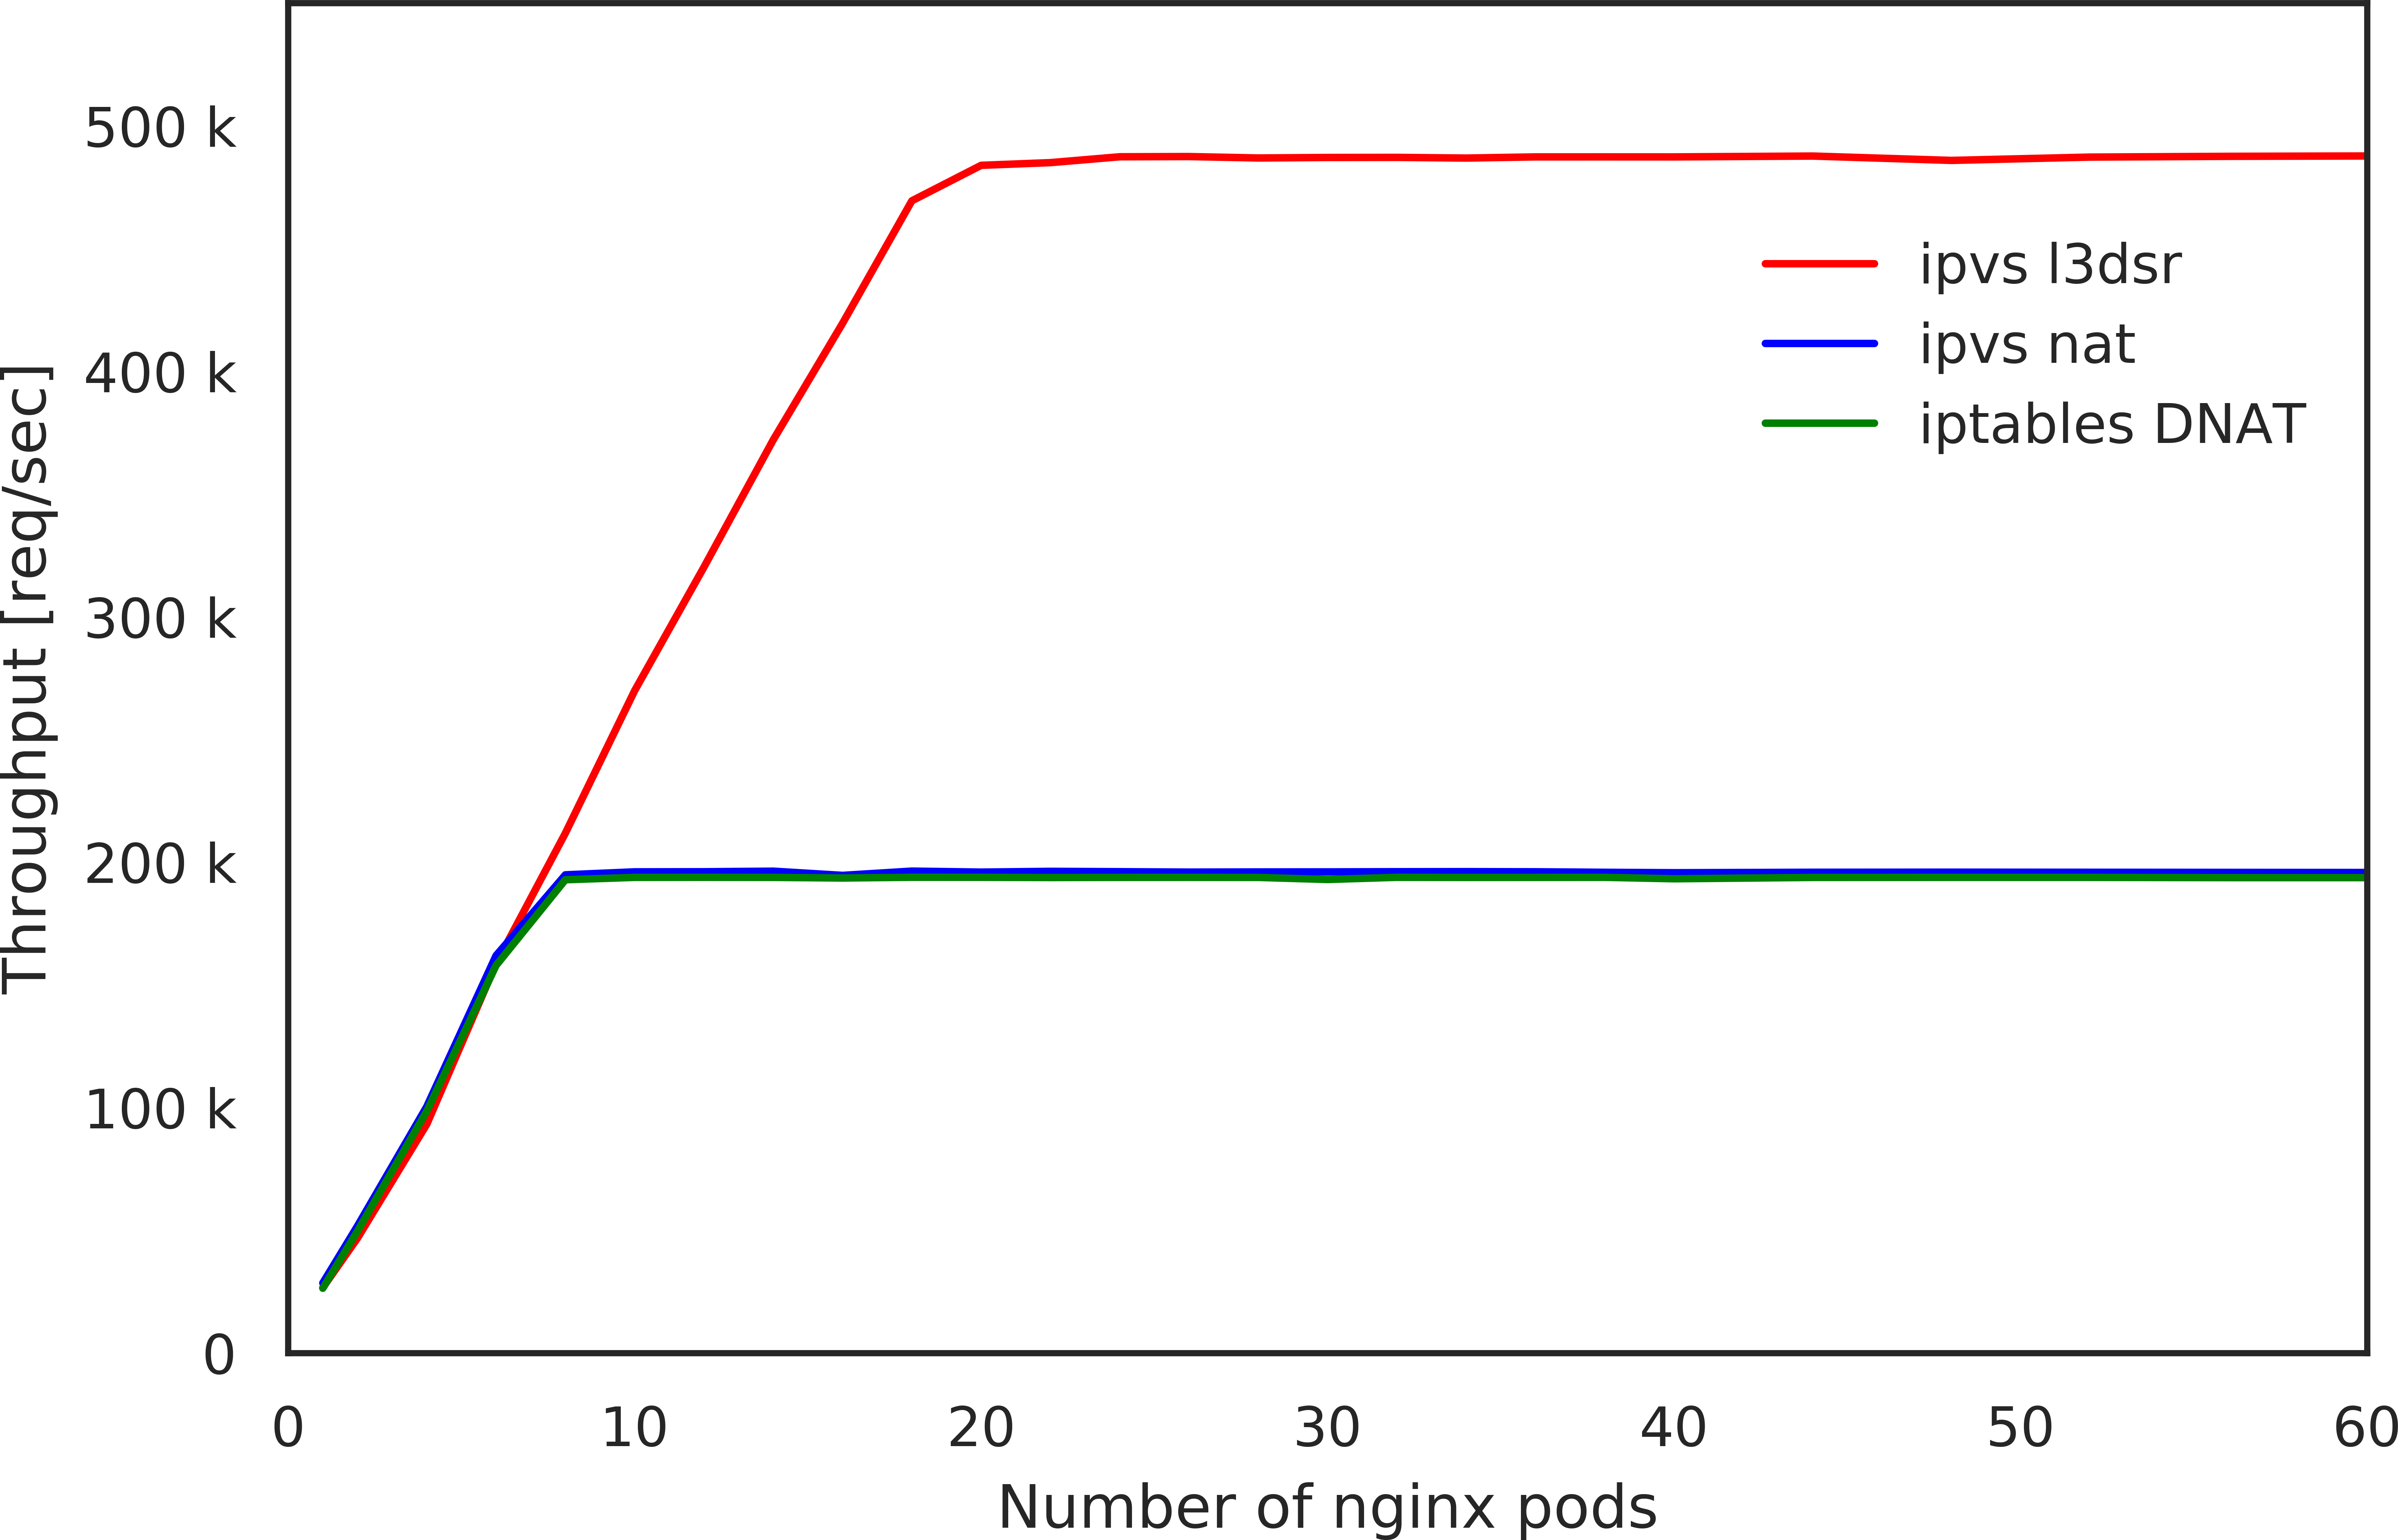
\includegraphics[width=0.8\columnwidth]{Figs/ipvs_l3dsr_1g.png}
  \caption{Throughput of ipvs l3dsr @1Gbps.}
  \label{fig:ipvs_l3dsr_1g.png}
\end{figure}

The author carried out throughput measurement using the physical setup shown in Figure~\ref{fig:bench_1g_l3dsr}.
Figure~\ref{fig:ipvs_l3dsr_1g.png} shows the throughput of the ipvs-tun, conventional ipvs (after here the author call it ipvs-nat) and iptables DNAT.
As can be seen in the figure, while the performance levels for ipvs-nat and iptables DNAT exactly match, the performance levels for ipvs-tun is greatly improved, e.g., 1.5 times larger saturated throughput than for ipvs-nat and iptables DNAT cases.

\FloatBarrier

\section{ECMP redundancy}

This section discusses the redundancy and scalability of the proposed load balancers.
The ECMP technique is expected to make the load balancers redundant and scalable since all the load balancer containers act as active.
The whole system is resilient to a single failure of load balancer container.
Also since multiple of load balancers can be utilized simultaneously, it is expected that the throughput of the total system is increased significantly.
In order to evaluate these characteristics of the ECMP technique,
the author examined if the ECMP routing table is updated correctly when multiple of the load balancer {\em pods} are started.
After that, in order to explore the scalability, the author also measured the throughput of the cluster of load balancers.
Finally, the author examined how quick those ECMP routing table updates are.
The following sections explain the evaluation in detail.

\subsection{Evaluation method}

\begin{figure}[b]
  \centering
    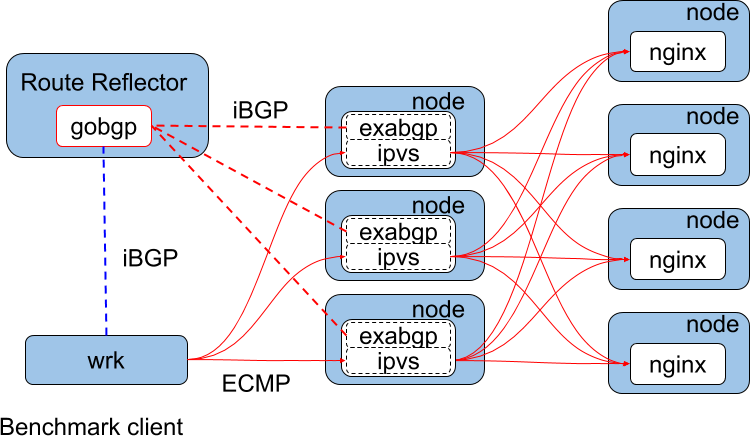
\includegraphics[width=0.9\columnwidth]{Figs/lb_ecmp_schem}
    \caption{Experimental setups.}
    \label{fig:lb_ecmp_schem}
\end{figure}

\begin{table}[b]
  \centering
  \begin{tabular}{ll}
    \hline \\
    \multicolumn{2}{l}{[Hardware Specification]}   \\
    & CPU: Xeon E5-2450 2.10GHz x 8 (with Hyper Threading) \\
    & Memory: 32GB \\
    & NIC: Broadcom BCM5720 Giga bit \\
    & (Node x 6, Load Balancer x 4) \\
    & \\
    & CPU: Xeon E5-2450 2.10GHz x 8 (with Hyper Threading) \\
    & Memory: 32GB \\
    & NIC: Intel X550 \\
    & (Client x 1) \\
    & \\
    \multicolumn{2}{l}{[Node Software]}  \\
    & OS: Debian 9.5, linux-4.16.8 \\
    & Kubernetes v1.5.2 \\
    & flannel v0.7.0 \\
    & etcd version: 3.0.15 \\
    & \\
    \multicolumn{2}{l}{[Container Software]}   \\
    & Keepalived: v1.3.2 (12/03,2016) \\
    & nginx : 1.15.4(web server) \\
    \\ \hline
  \end{tabular}
  \caption{Hardware and software specifications.}
  \label{tab:ecmp-hw_sw_spec}
\end{table}

Figure~\ref{fig:lb_ecmp_schem} shows the schematic diagram of the experimental setup.
And Table~\ref{tab:ecmp-hw_sw_spec} summarizes hardware and software specifications for the experiments.
%
Multiple {\em pods} are deployed on multiple nodes in the Kubernetes cluster.
In each {\em pod}, an nginx web server pod that returns the IP address of the {\em pod} are running.
There are multiple nodes for load balancers and on each of the nodes, single load balancer {\em pod} is deployed.
Each load balancer {\em pod} consists of both an ipvs container and an exabgp container.
The routing table of the benchmark client is updated by BGP protocol through a route reflector.

Using these hardware and software setups the following four types of evaluations have been carried out;
1) Evaluation of ECMP functionality. The author examined if ECMP routing table is correctly updated.
2) Evaluation of the scalability. The author evaluated how throughput is improved by running multiple ipvs pods simultaneously.
3) Evaluation of ECMP response. The author evaluated the delay between the time ipvs pods are started or stopped until the time ECMP routing table reflected the change.


The throughputs are measured using wrk in the same manner as in Chapter~\ref{chapter:portablelb}.
Notable differences from the previous throughput experiment in Figure~\ref{fig:benchmark-setup} are;
There four nodes for load balancers instead of one.
Also, the 10 Gbps NIC is used for the benchmark client since for scalability experiment, there are multiple of ipvs container load balancers that can fill up 1 Gbps bandwidth.
Some of the software has also been updated to the most recent versions at the time of the experiment.

\FloatBarrier

\subsection{Reults}

\subsubsection{ECMP functionality}

\begin{table}[h]

  \begin{subtable}{.9\textwidth}
  \centering
  \begin{tabular}{l}
    \hline 
    10.1.1.0/24 via 10.0.0.106 dev eth0 proto zebra metric 20 \\
    \hline
  \end{tabular}
  \caption{With single load balancer {\em pod}.}
  \label{tab:single}
\end{subtable}

\begin{subtable}{.9\textwidth}
  \centering
  \begin{tabular}{ll}
    \hline
    \multicolumn{2}{l}{10.1.1.0/24 proto zebra metric 20 } \\
    \hspace{15 mm}
    & nexthop via 10.0.0.105  dev eth0 weight 1 \\
    & nexthop via 10.0.0.106  dev eth0 weight 1 \\
    & nexthop via 10.0.0.107  dev eth0 weight 1 \\
    \hline
  \end{tabular}
  \caption{With three load balancer {\em pod}s.}
  \label{tab:three}
\end{subtable}

\begin{subtable}{.9\textwidth}
  \centering
  \begin{tabular}{ll}
    \hline
    \multicolumn{2}{l}{10.1.1.0/24 pro to zebra metric 20 } \\
    \hspace{15 mm}
    & nexthop via 10.0.0.107  dev eth0 weight 1 \\
    & nexthop via 10.0.0.105  dev eth0 weight 1 \\
    & nexthop via 10.0.0.106  dev eth0 weight 1 \\
    \multicolumn{2}{l}{10.1.2.0/24 proto zebra metric 20 } \\
    \hspace{15 mm}
    & nexthop via 10.0.0.107  dev eth0 weight 1 \\
    & nexthop via 10.0.0.106  dev eth0 weight 1 \\
    \hline
  \end{tabular}
  \caption{For a service with three load balancer {\em pod}s and a service with two load balancer {\em pod}s.}
  \label{tab:double_svc}
\end{subtable}

\caption{ECMP routing tables.}
\label{tab:exabgp_routing_table}
\end{table}

First, the author examined ECMP functionality by monitoring the routing table on the benchmark client.
Table~\ref{tab:exabgp_routing_table}~(\subref{tab:single}) shows the routing table entry on the router when a single load balancer pod existed.
From this entry, we can tell that packets toward 10.1.1.0/24 are forwarded to 10.0.0.106 where the load balancer pod is running.
There is also a keyword, zebra, which indicates that zebra controls this routing rule.

When the number of the load balancer pods was increased to three, the routing table becomes to have entries in Table~\ref{tab:exabgp_routing_table}~(\subref{tab:three}).
There are three next hops towards 10.1.1.0/24 each of which being the node where the load balancer pods are running.
The weights of the three next-hops are equal, i.e., 1.
The update of the routing entry was almost instant as the author increased the number of the load balancers.

Table~\ref{tab:exabgp_routing_table}~(\subref{tab:double_svc}) shows the case where the author additionally started new service with two load balancer pods with service addresses in 10.1.2.0/24 range.
It was possible to accommodate two different services with different IP addresses, one with three load balancers and the other with two load balancers on a group of nodes, 10.0.0.105, 10.0.0.106 and 10.0.0.107.
The update of the routing entry was almost instant as the author started the load balancers for the second service.

\FloatBarrier

\subsubsection{Scalability}

\begin{figure}[h]
  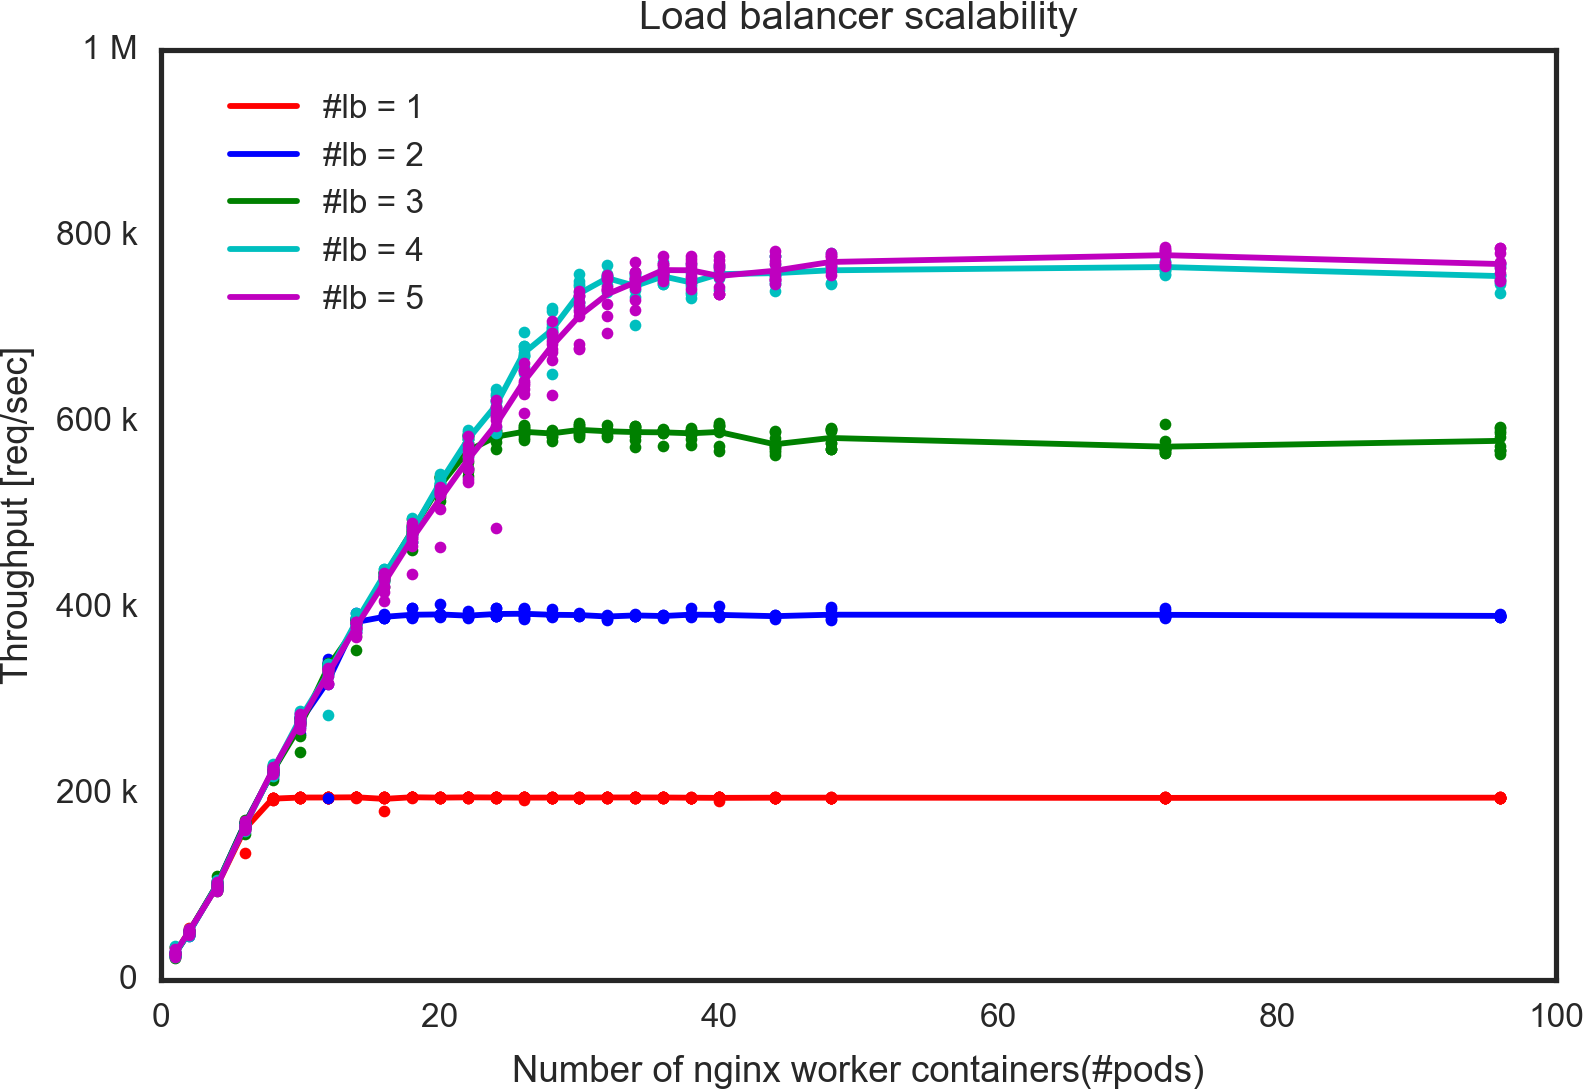
\includegraphics[width=0.9\columnwidth,left]{Figs/ecmp_lb_cubic}
  \caption{Throughput of ECMP redundant load balancer.}
The throughputs are measured for a single load balancer(lb x1), two(lb x2), three(lb x3) and four(lb x4) load balancers. 

\label{fig:ecmp_lb_cubic}
\end{figure}

The throughput measurement was also carried out to show that ECMP technique increases the throughput as the number of the load balancers is increased.
Figure~\ref{fig:ecmp_lb_cubic} shows the results of the measurements.
There are four solid lines in the figure, each corresponding the throughput result when there are one through four of the proposed load balancers.

As can be seen in the figure, as we increased the number of the pod the throughput increased linearly to a certain level after which it saturated.
The saturated levels, i.e. performance levels, depend on the number of the ipvs load balancer pods (lb x 1 being the case with one ipvs pods, and lb x2 being two of them and as such).
The performance levels increase linearly as we increase the number of the load balancers.
The performance level did not scale further when the number of load balancers was increased more than four.
This was because the performance of the benchmark client was hitting the ceiling, i.e., the CPU usage was 100\% when the total throughput was around 780k [req/sec].
The author expects that replacing the benchmark client with more powerful machines will further improve the performance level this system.

\FloatBarrier

\subsubsection{Response}

\begin{figure}[t]
  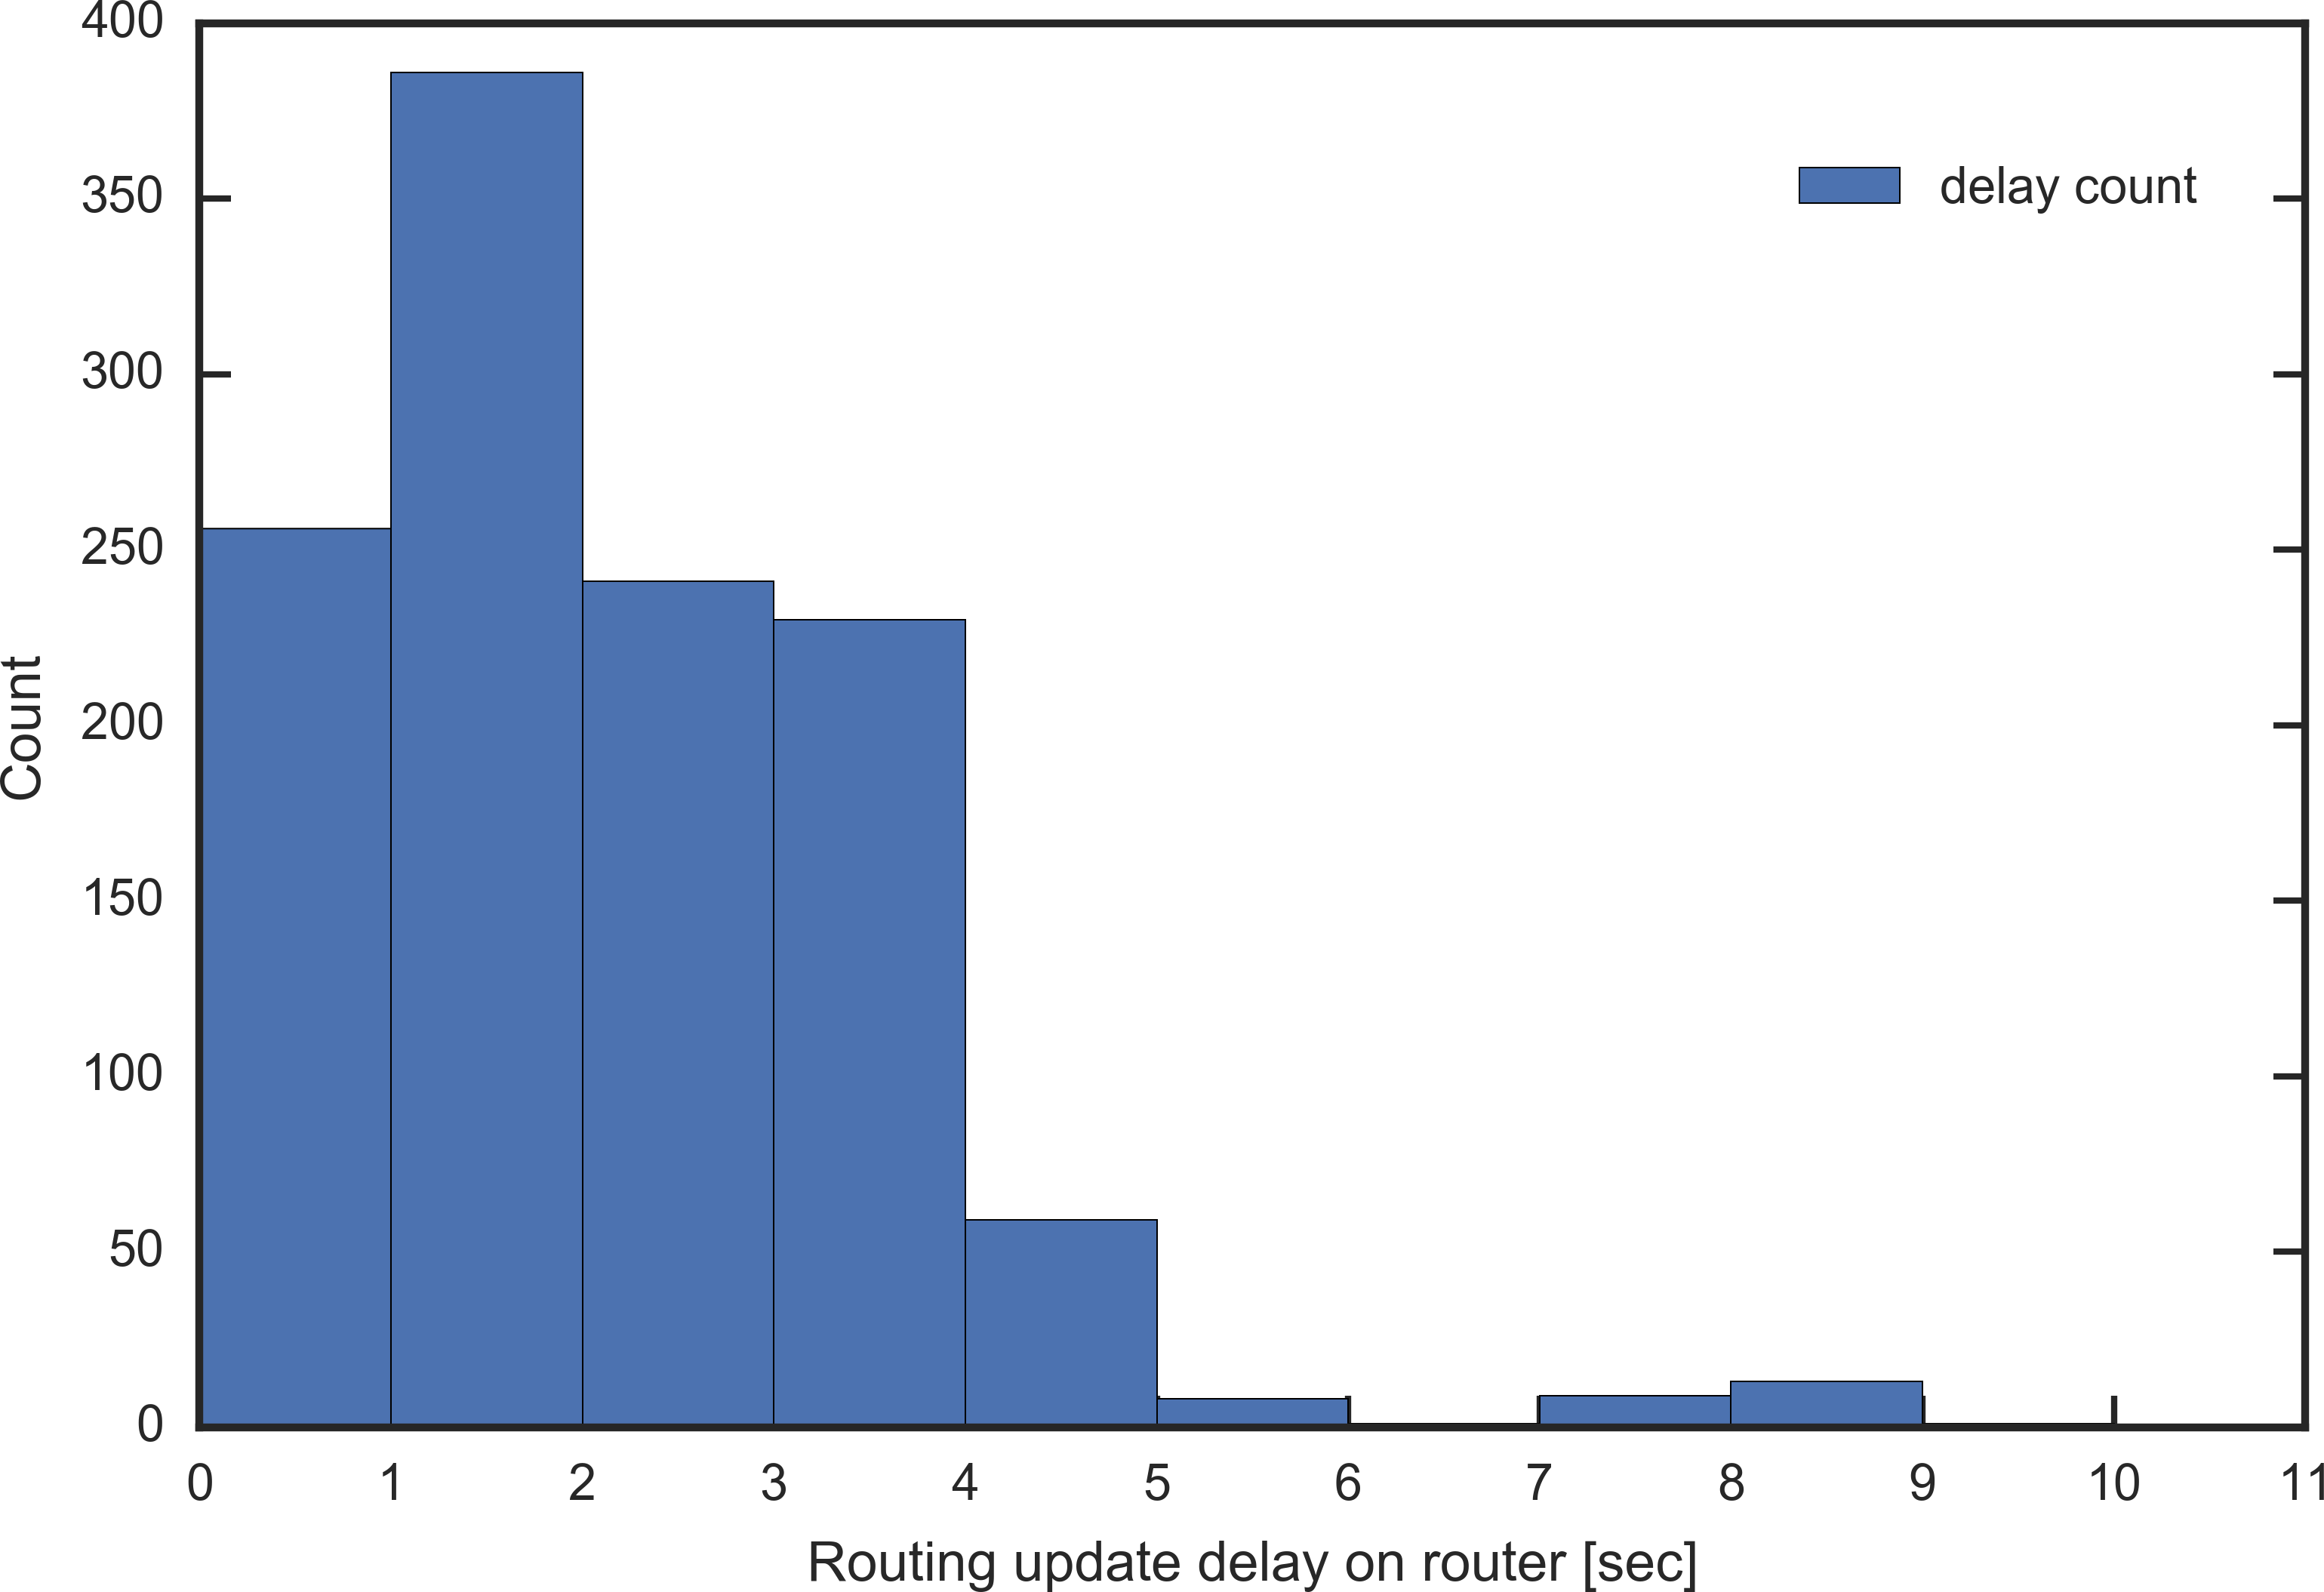
\includegraphics[width=0.9\columnwidth,left]{Figs/ecmp_delay_histgram}
  \caption{A histogram of the ECMP update delay.}
This shows the delays until the number of running ipvs pods is reflected into the routing table on the benchmark client,
when the number of the ipvs pods is changed randomly every 60 seconds for 20 hours.
  \label{fig:ecmp_delay_histgram}
\end{figure}

Figure~\ref{fig:ecmp_delay_histgram} shows the histogram of the ECMP update delay.
The author measured the delays until the number of running ipvs pods is reflected into the routing table on the benchmark client.
The number of the ipvs pods is changed randomly every 60 seconds for 20 hours.
As we can see from the figure, most of the delays are within 6 seconds, and the largest delay was 10 seconds.
We can say that ECMP routing update in our proposed architecture is quick enough.

\begin{figure}[t]
  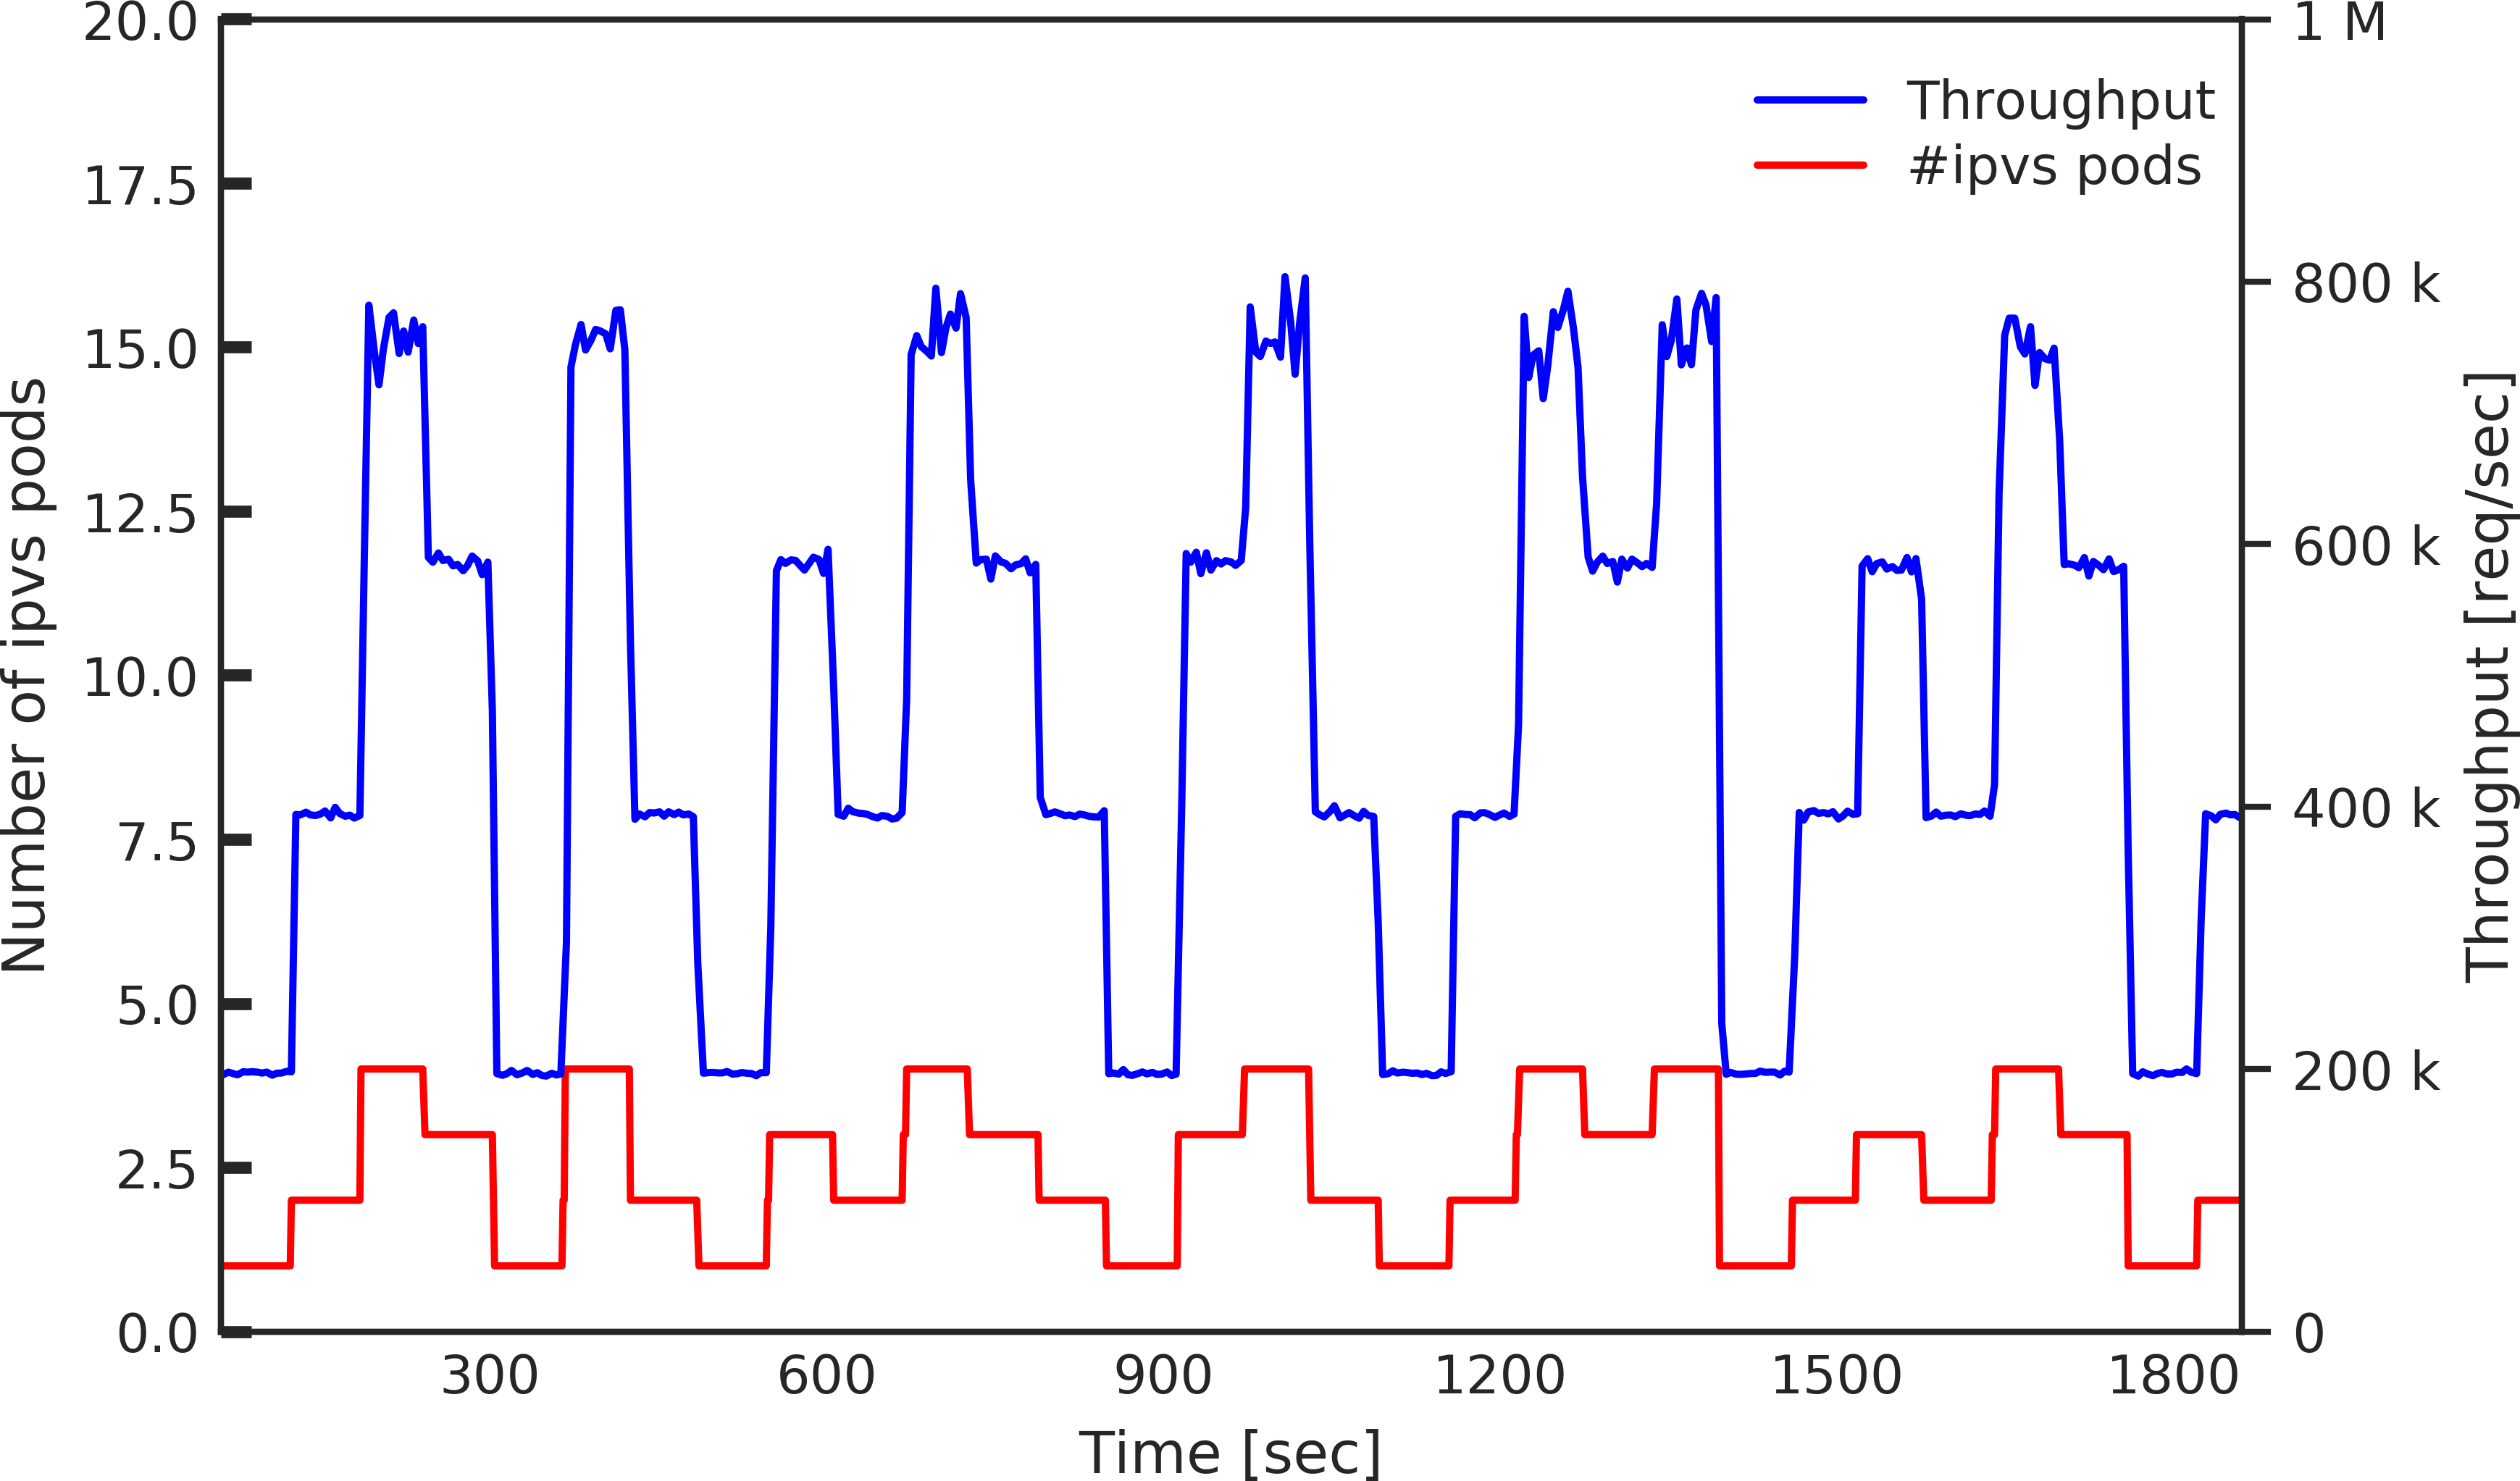
\includegraphics[width=0.98\columnwidth,left]{Figs/ecmp_response}
  \caption{Throughput responsiveness.}
This shows the throughput responsiveness when the number of the load balancers was changed randomly in every 60 seconds. 
  \label{fig:ecmp_response}
\end{figure}

Figure~\ref{fig:ecmp_response} shows the throughput measurement results when the number of the load balancers was periodically changed. 
The red line in the figure shows the number of the ipvs load balancer pods, which was changed randomly in every 60 seconds.
The blue line corresponds to the resulting throughput.
As we can see from the figure, the blue line nicely follows the shape of the red line.
This indicates that new load balancers are immediately utilized after they are created.
It also indicates that after removing some load balancers, the traffic to them is immediately directed to the existing load balancers.

\FloatBarrier


\section{Cloud experiment
%%  [Add experimental conditions for GCP and AWS]
}

\subsection{Method}

\subsection{Results}

\begin{figure}[t]
  \centering
  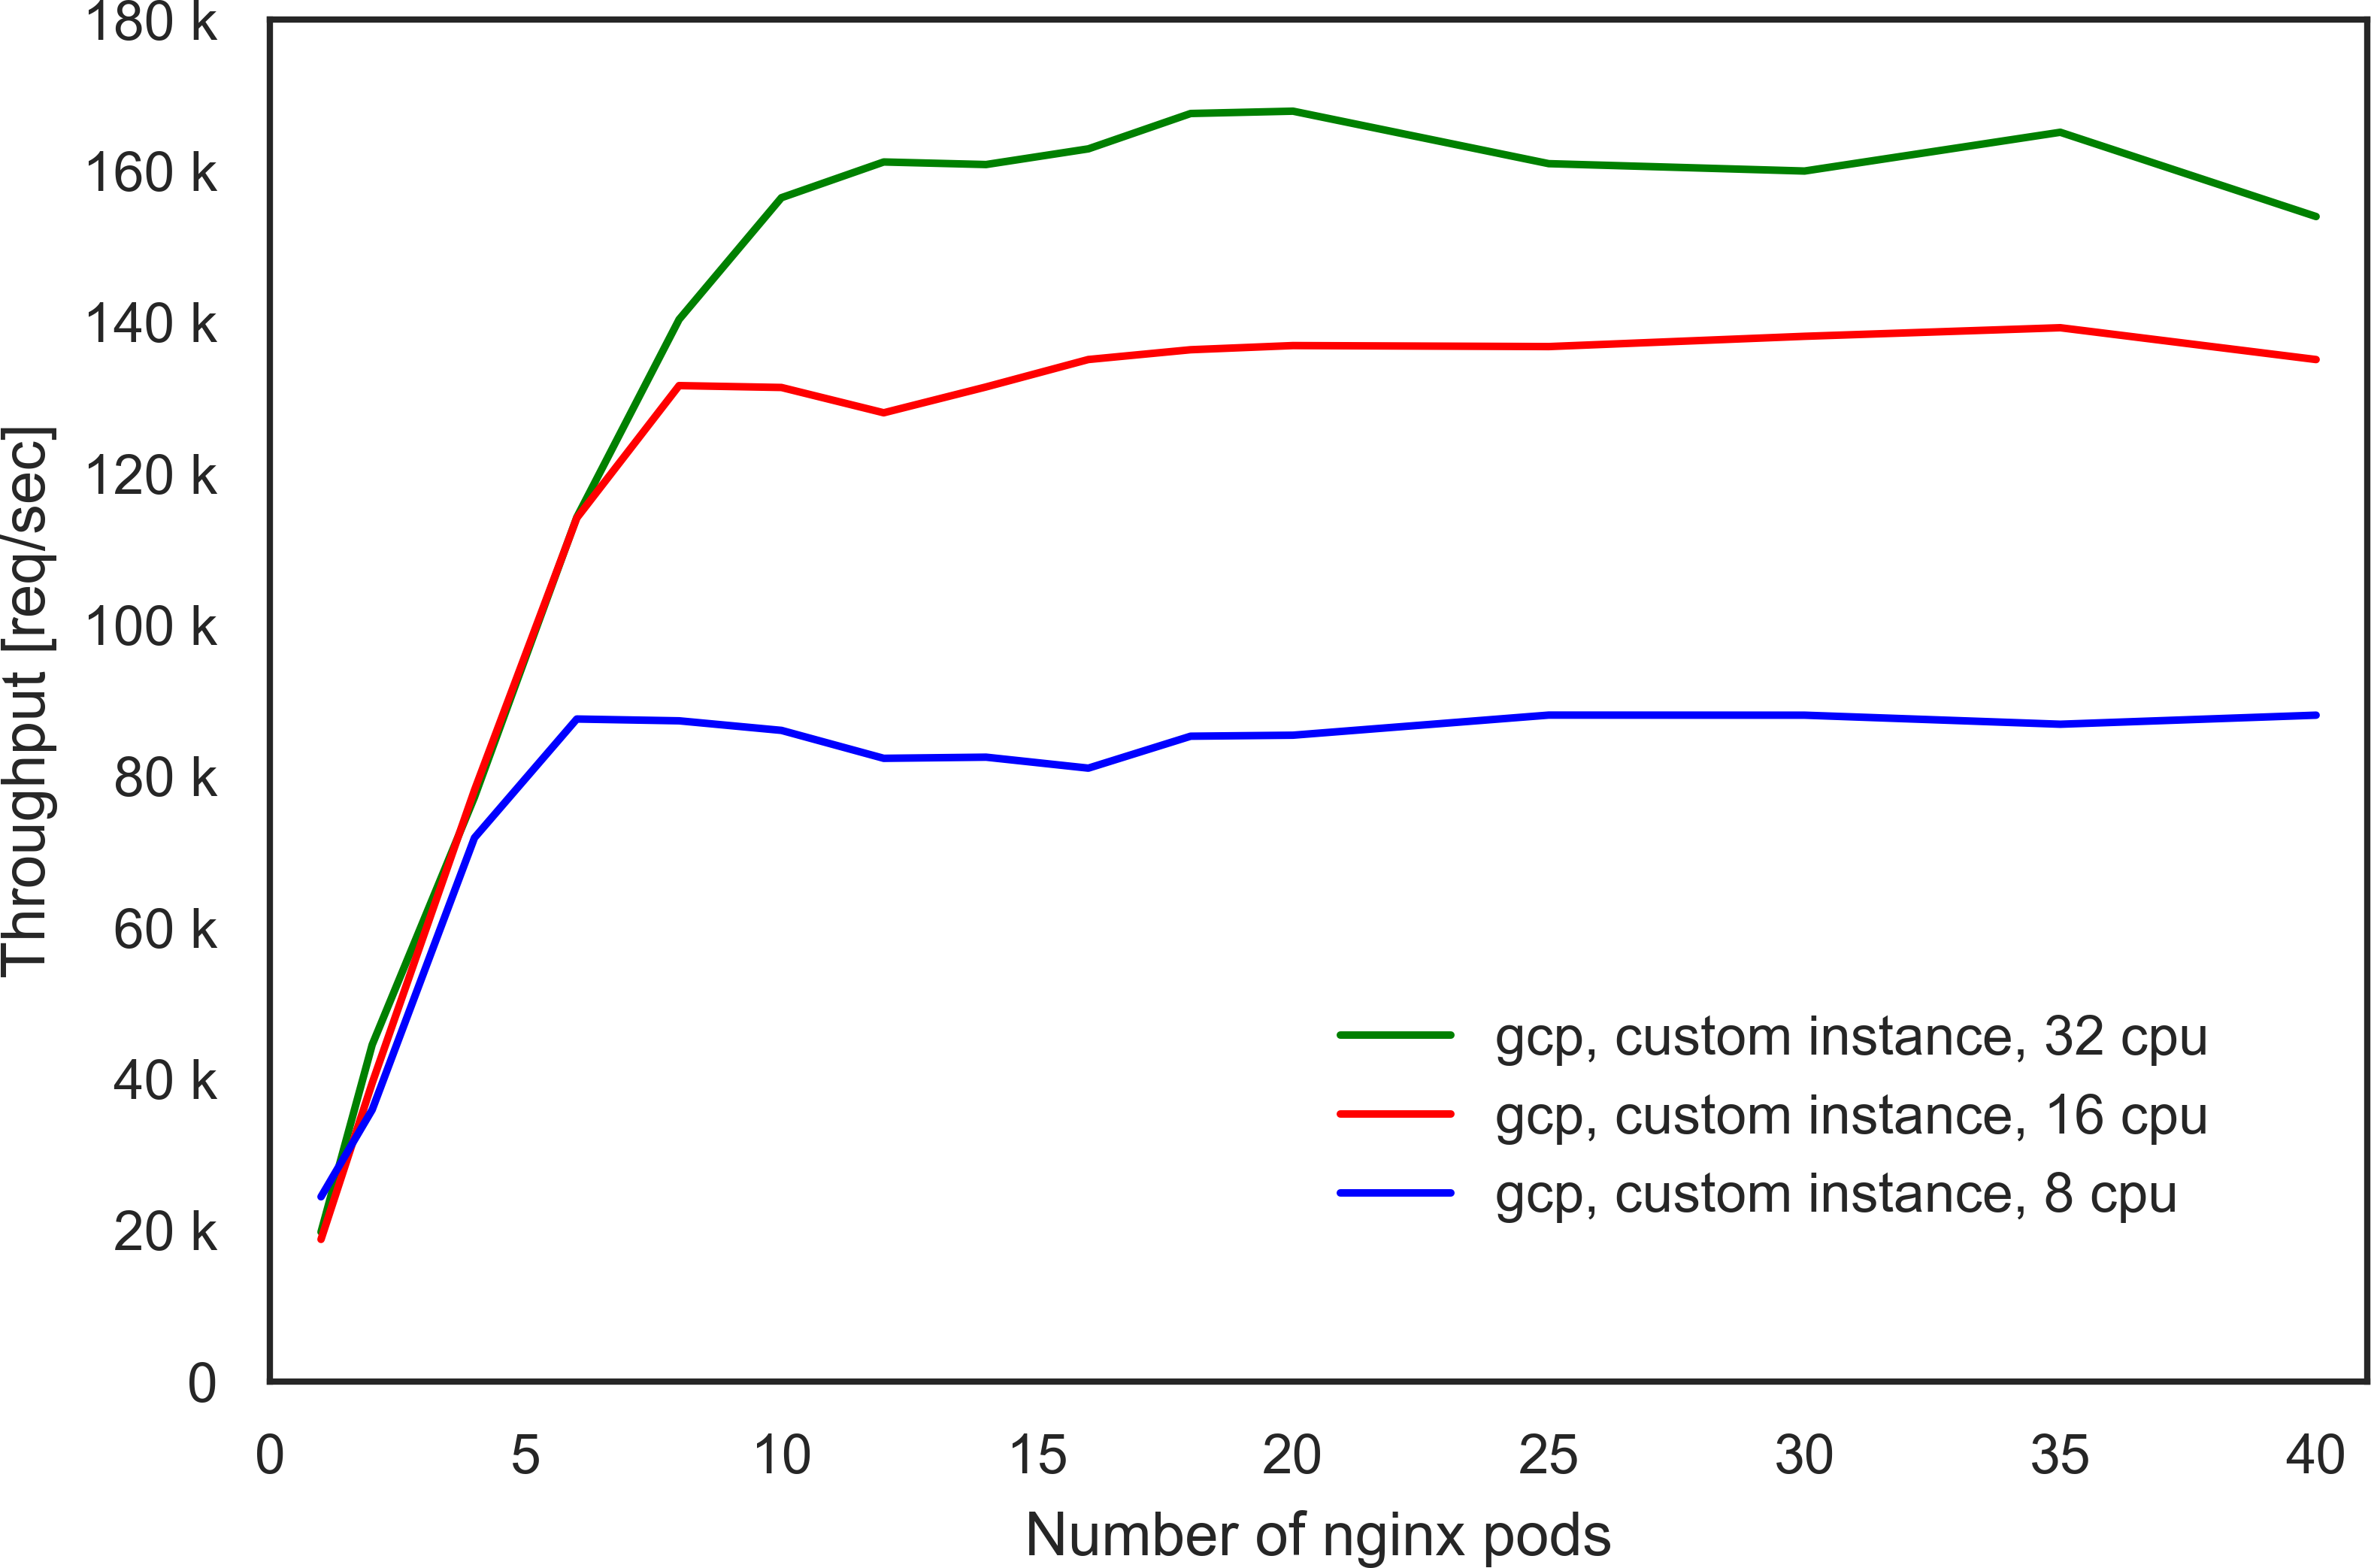
\includegraphics[width=0.8\columnwidth]{Figs/gcp_all_tp}
  \caption{GCP}
  \label{fig:gcp_all_ieice}
\end{figure}

\begin{figure}[t]
  \centering
  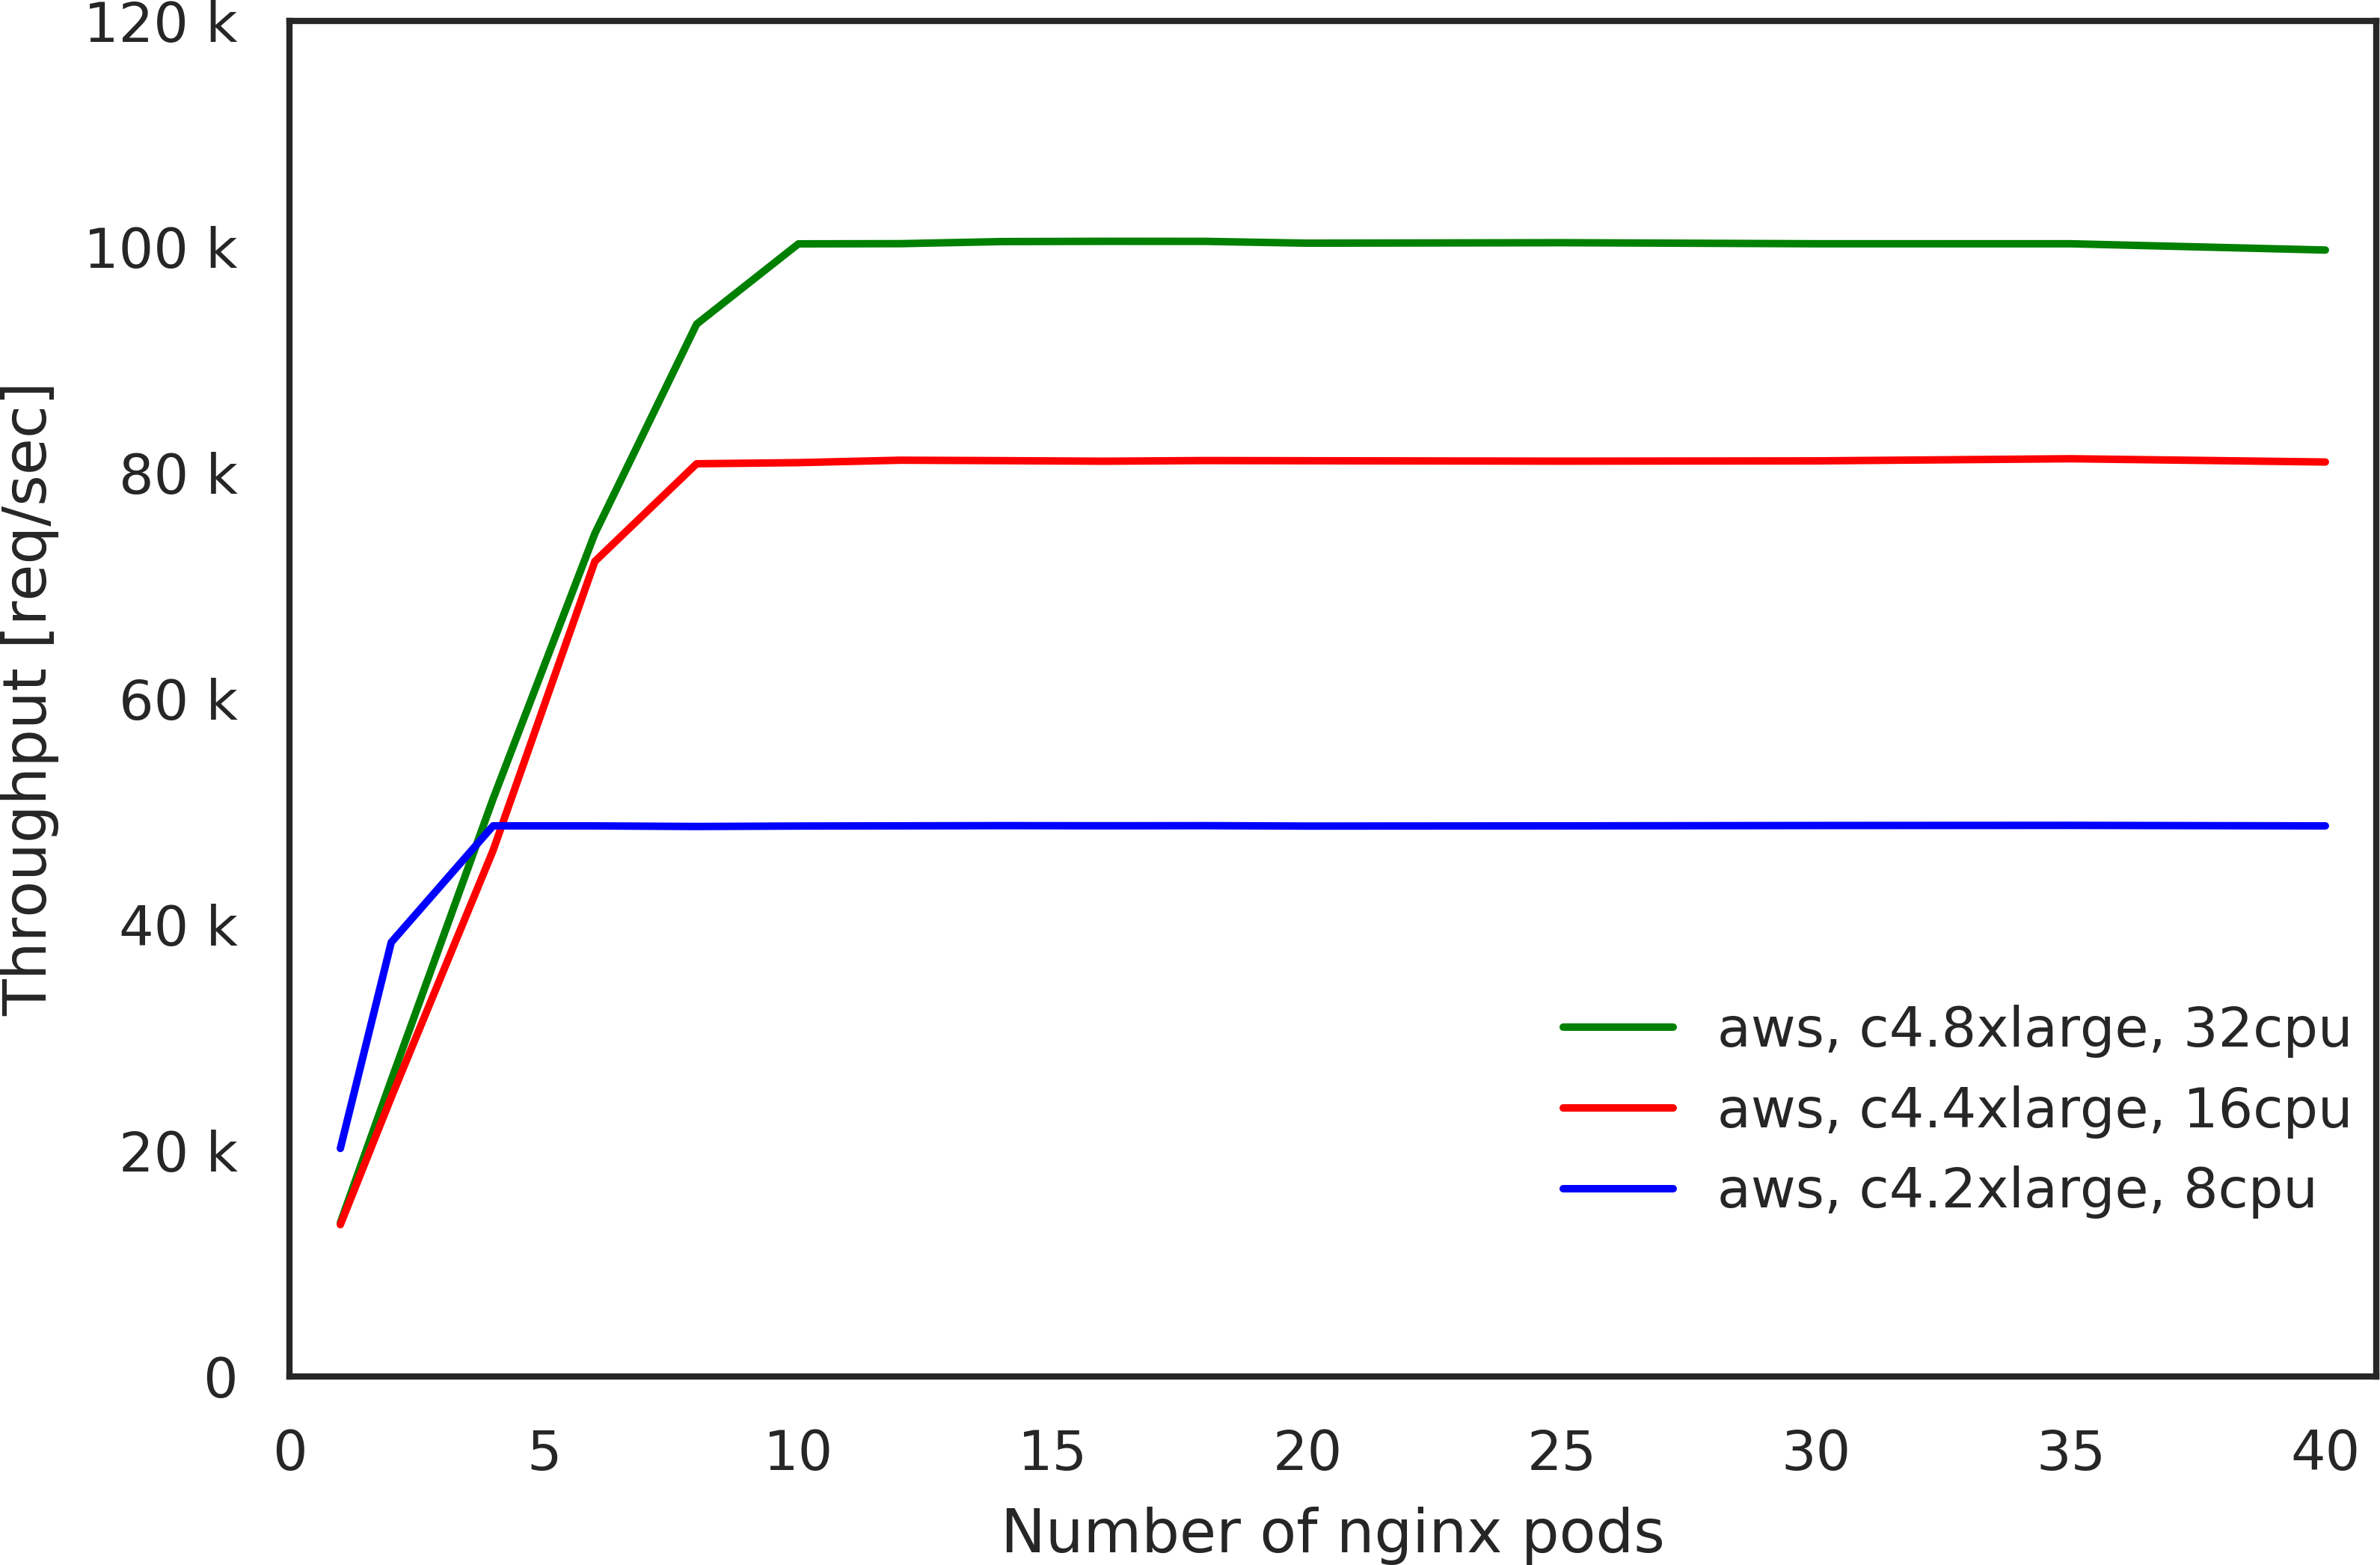
\includegraphics[width=0.8\columnwidth]{Figs/aws_c4_tp}
  \caption{AWS with Node x 6, Client x 1, Load balancer x 1. Custom instance. }
  \label{fig:aws_c4_ieice}
\end{figure}

So far, it has been shown that the proposed ipvs-nat load balancer in a container has equivalent throughput, and the proposed ipvs-tun load balancer in a container has even better throughputs.
In this section, the author shows that the proposed load balancer is portable by showing that it can be run in cloud environments, and also shows that it has the same behavior as in on-premise data centers.

Figure~\ref{fig:gcp_all_ieice} and Figure~\ref{fig:aws_c4_ieice} show the load balancer performance levels that are measured in GCP and AWS, respectively.
For both environments, the author measured throughput with several conditions of CPU counts, since the machine specifications can be easily changed in the cases of cloud environments.
Both results show similar characteristics as the experiment in an on-premise data center in Figure~\ref{fig:ipvs_mcore_proccessing}, where throughput increases linearly to a certain saturation level that is determined by utilized CPU core count.
In other words, it indicates that the proposed load balancer can be run in cloud environments and also functions properly.

It seems that CPU counts determine the load balancer's throughput saturation levels.
The actual throughput numbers are smaller than those of the load balancers in on-premise data centers.
This may be because the physical servers in on-premise data center outperform the VMs in a cloud environment, or because network bandwidth is smaller and is limited based on the type of instances.
A detailed analysis is further required in the future to clarify which factor limits the throughput in the case of the cloud environment.
Nonetheless, we can say that the proposed ipvs load balancers can be run in both GCP and AWS, and the behavior is the same with the load balancers in on-premise data centers.


\FloatBarrier

\section{Summary}

\subsection{singl lb}

In this chapter portability and performance level of proposed load balancer in 1 Gbps network environments has been discussed.
The throughput levels of a load balancer are dependent on settings for multicore packet processing.
It is clear that the case that utilizes all of the CPU cores better performs than the case with only four CPU cores utilized.
It is better to use as many CPU cores as possible for packet processing.
The throughput levels are also very dependent on the back end mode of the flannel overlay network.
The host-gw mode where no tunneling is used resulted in the best performance level.

The performance levels of ipvs-nat, iptables DNAT and nginx have also been compared.
The proposed ipvs-nat load balancer in the container had the same performance level as load balancing function of iptables DNAT.
Furthermore, in the case of L3DSR setup, the performance level of ipvs-tun load balancer has about 1.5 times larger than that of ipvs-nat and iptables DNAT.

It is also shown that the proposed load balancer can be run in GCP and AWS.
The behavior of the proposed load balancer in those cloud environments is the same as that in the on-premise data center.
The author concludes that the proposed load balancer is portable and outperforms the existing iptables DNAT load balancers in 1 Gbps network environments.


\subsection{ECMP}

In this chapter, the redundancy and scalability of the proposed load balancers have been discussed.
The author verified that ECMP routing table was properly created in the experimental system.
The update of the ECMP routing table was quick enough, i.e., within 10 seconds, throughout 20 hours experiment and the routing table was always correct.
The scalability of the load balancer was also examined and it has been found that maximum performance levels scaled linearly as the number of the load balancer pods was increased to four.
The maximum throughput level obtained through the experiment was 780k [req/sec], which is limited due to the maximum CPU performance of the benchmark client rather than the performance of the load balancer cluster.


